\documentclass{report}
\usepackage[T1]{fontenc} % Fonts T1
\usepackage[utf8]{inputenc} % Input UTF8
\usepackage[backend=biber, style=ieee]{biblatex} % for using bibliography
\usepackage{csquotes}
\usepackage[english]{babel} %Using english llanguage
\usepackage{blindtext} % Generating text automatically
\usepackage[printonlyused]{acronym}
\usepackage{hyperref} % for autoref
\usepackage{graphicx}
\usepackage{indentfirst}
\usepackage{comment}
\usepackage{copyrightbox}


\bibliography{bibliography}


\begin{document}
%%
% Definitions
%
\def\titledoc{ART}
\def\datedoc{DATE}
\def\authors{Rodrigo Ribeiro, Zuzanna Sikorska}
\def\authorscontacts{(113711) rodrigo.ribeiro@ua.pt, (112018) zuzanna.sikorska@ua.pt}
\def\version{Version 1.0}
\def\department{Dept. de Eletrónica, Telecomunicações e Informática}
\def\company{Universidade de Aveiro}
\def\logo{img/ua.pdf}
\def\repository{infor2022-ap-g25}
%
%%%%%% COVER %%%%%%
%
\begin{titlepage}

\begin{center}
%
\vspace*{50mm}
%
{\Huge \titledoc}\\ 
%
\vspace{10mm}
%
{\Large \company}\\
%
\vspace{10mm}
%
{\LARGE \authors}\\ 
%
\vspace{30mm}
%
\begin{figure}[h]
\center
\includegraphics{\logo}
\end{figure}
%
\vspace{30mm}
\end{center}
%
\begin{flushright}
\version
\end{flushright}
\end{titlepage}

%%  Title Page %%
\title{%
{\Huge\textbf{\titledoc}}\\
{\Large \department\\ \company}
}
%
\author{%
    \authors \\
    \authorscontacts \\
    \repository
}
%
\date{\today}
%
\maketitle

\pagenumbering{roman}

%%%%%% SUMMARY %%%%%%
\begin{abstract}

\textbf{Types of art}  - Art is a creative process some go through to express their emotions, send a message, raise awareness and present ideas. Art can be devided in three sections: visual art - which includes painting, sculptures, architecture - performing art - including dance, music and theatre - and literary art - fiction, drama and poetry.


\textbf{Art movements} - Art is a well known concept present throughout all of human history. As humans evolved and power structures were developed, they heavily influenced societies along history and various movements were created and each of them is rensponsible for having their own style. The report includes ten different art movements which are debatably the most impactful in all of human history. The third chapter will explain five important movements during the middle ages until the the modern era, while the fourth chapter englobes more recent art movements, like street art and social realism art.

\end{abstract}

%%%%%% Acknowledgments %%%%%%
% According to glisc should appear after conclusions ...

\begin{comment}
\renewcommand{\abstractname}{Acknowledgments}
\begin{abstract}
Any acknowledgments.
Comment block if no acknowledgments are due.
\end{abstract}
\end{comment}

\tableofcontents
% \listoftables     % descomentar se necessário
\listoffigures    % descomentar se necessário


%%%%%%%%%%%%%%%%%%%%%%%%%%%%%%%
\clearpage
\pagenumbering{arabic}

%%%%%%%%%%%%%%%%%%%%%%%%%%%%%%%%
\chapter{Introduction}
\label{chap.intro}

Art is an abstract. It surrounds everyone in a indistinguishable way. Art is reserved only for people, it distinguish all human beings from other living creatures. The ability of creating something only for aesthetic reasons is something unique, but on the other hand it also becomes underestimated in the world based on career and money. This document focuses on dividing the undefined art term into a few cathegories providing the comprehensive explanation of each of them. The aim is to put flesh on the details of the most found art forms and styles and to make them more understandable for ordinary man.

This document is divided into five chapters.
After this introduction,
in \autoref{chap.forms_of_art} the forms of art are presented and exhaustively analysed,
in \autoref{chap.influential_art_movements} the most influential art movements are discussed
and in \autoref{chap.modern_art_movements} the focus is on the most recently discovered styles.
Finally, in \autoref{chap.conclusions} the conclusions of the work.


\chapter{Forms of Art}
\label{chap.forms_of_art}

\section{Painting}

Painting is a visual form of art that usually consists on the application of paint on a support - canvas, paper, glass, walls, etc. There's many different tools - most commonly used are spatulas, brushes, pens, pencils - that can be used to apply paint, color or pigment to accomplish different types of paintings. It fundamentally consists on viewing figures on a two dimensional matrix. 

Although these are very popular methods nowadays, painting as a form of art has evolved for many years, going back thousands of years to which scientists and researchers found a pig ilustrated in a cave and came to the conclusion that these cave paintings found in Leang Tedongnge, Indonesia, are at least 45500 years old (\autoref{fig:cavepainting}). Since they haven't invented paint these many years ago, they mostly used minerals to carve and leave colorful marks on the surface. Theres many other paintings that were found in caves, but all of them express the same thing - hunting - mostly big animals and barely any humans are in those drawings that aren't on hunting duties.

\begin{figure}[h]
\center
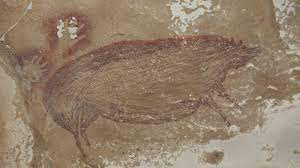
\includegraphics[height=4cm]{img/cavepainting}
\caption{Oldest cave painting found in Leang Tedongnge, Indonesia.}
\label{fig:cavepainting}
\end{figure}

Throughout human evolution, as religion rose in popularity all around the world, so did religious art, like Christian art, Hindu art, Islamic art and others. During these periods, many paintings were created with the objective of stimulating the mind of those that worship their Gods and Saints, since having a humanlike form was easier to perceive and understand them (\autoref{fig:religious-art}).

\begin{figure}[h]
\center
a) 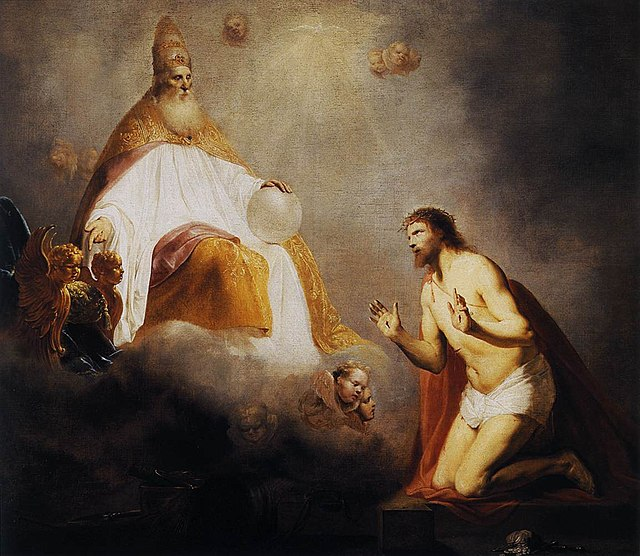
\includegraphics[height=3cm]{img/god}
b) 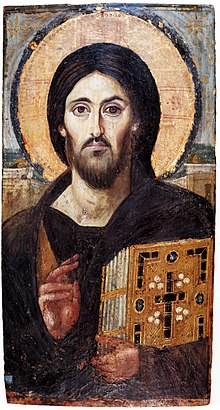
\includegraphics[height=3cm]{img/jesus}
c) 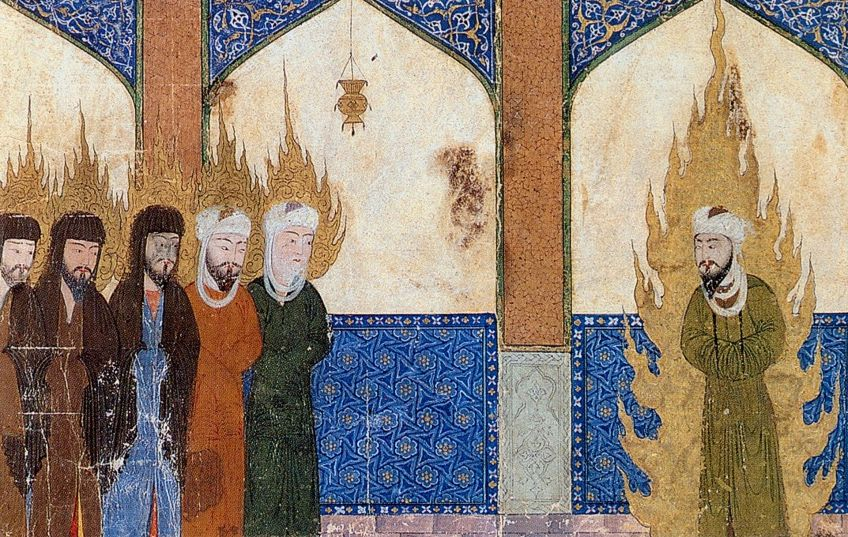
\includegraphics[height=3cm]{img/islampainting}
\caption{Historic paintings demonstraiting religion: a) God Inviting Christ to Sit on the Throne at His Right Hand by Pieter de Grebber,
b) Christ Pantocrator found in Monastery of St. Catherine on Mount Sinai, in Egypt, unknown author, c) Muhammad leading Abraham, Moses, and Jesus in prayer, unknown author}
\label{fig:religious-art}
\end{figure}

The manufactur of paintings will evolve simultaneously as technology progresses. During todays time, the most common type of art which is inert to us is digital art, present in our everyday lives, anywehre we go, which is deeply analyzed in the sub-chapter (\ref{sec.digital.art}).

\section{Sculpture}

Different sculpting techniques developed over the centuries allowed people to preserve the memory of their ancestors, perpetuate the achievements of previous generations, and were also an artistic expression of their identity. Monument sculpture has become, next to painting, a way to show the human body, it served to portray the faces of famous people, it allows sculptors to express their feelings and values that are valuable to them.

There are several types of classification of sculptures. They can be divided due to the shape for example full sculptures and reliefs. They can be free-standing or group sculptures, depicting heads, busts or full figures. A separate category are zoomorphic sculptures that present real or fantastic animals. The next group of sculptures are elements of flora, but also abstract forms created in the author's imagination \cite{BOOK:4}.

Creating wood sculptures is a popular carving technique that allows you to use the individual characteristics of a given piece of wood. Since there are no two identical branches or boughs, each woodwork is unique and difficult to imitate. One of the oldest wood carvings is believed to be the Shigir Idol, found near Yekaterinburg (\autoref{fig:shigir}).

\begin{figure}[h]
\center
\copyrightbox[b]{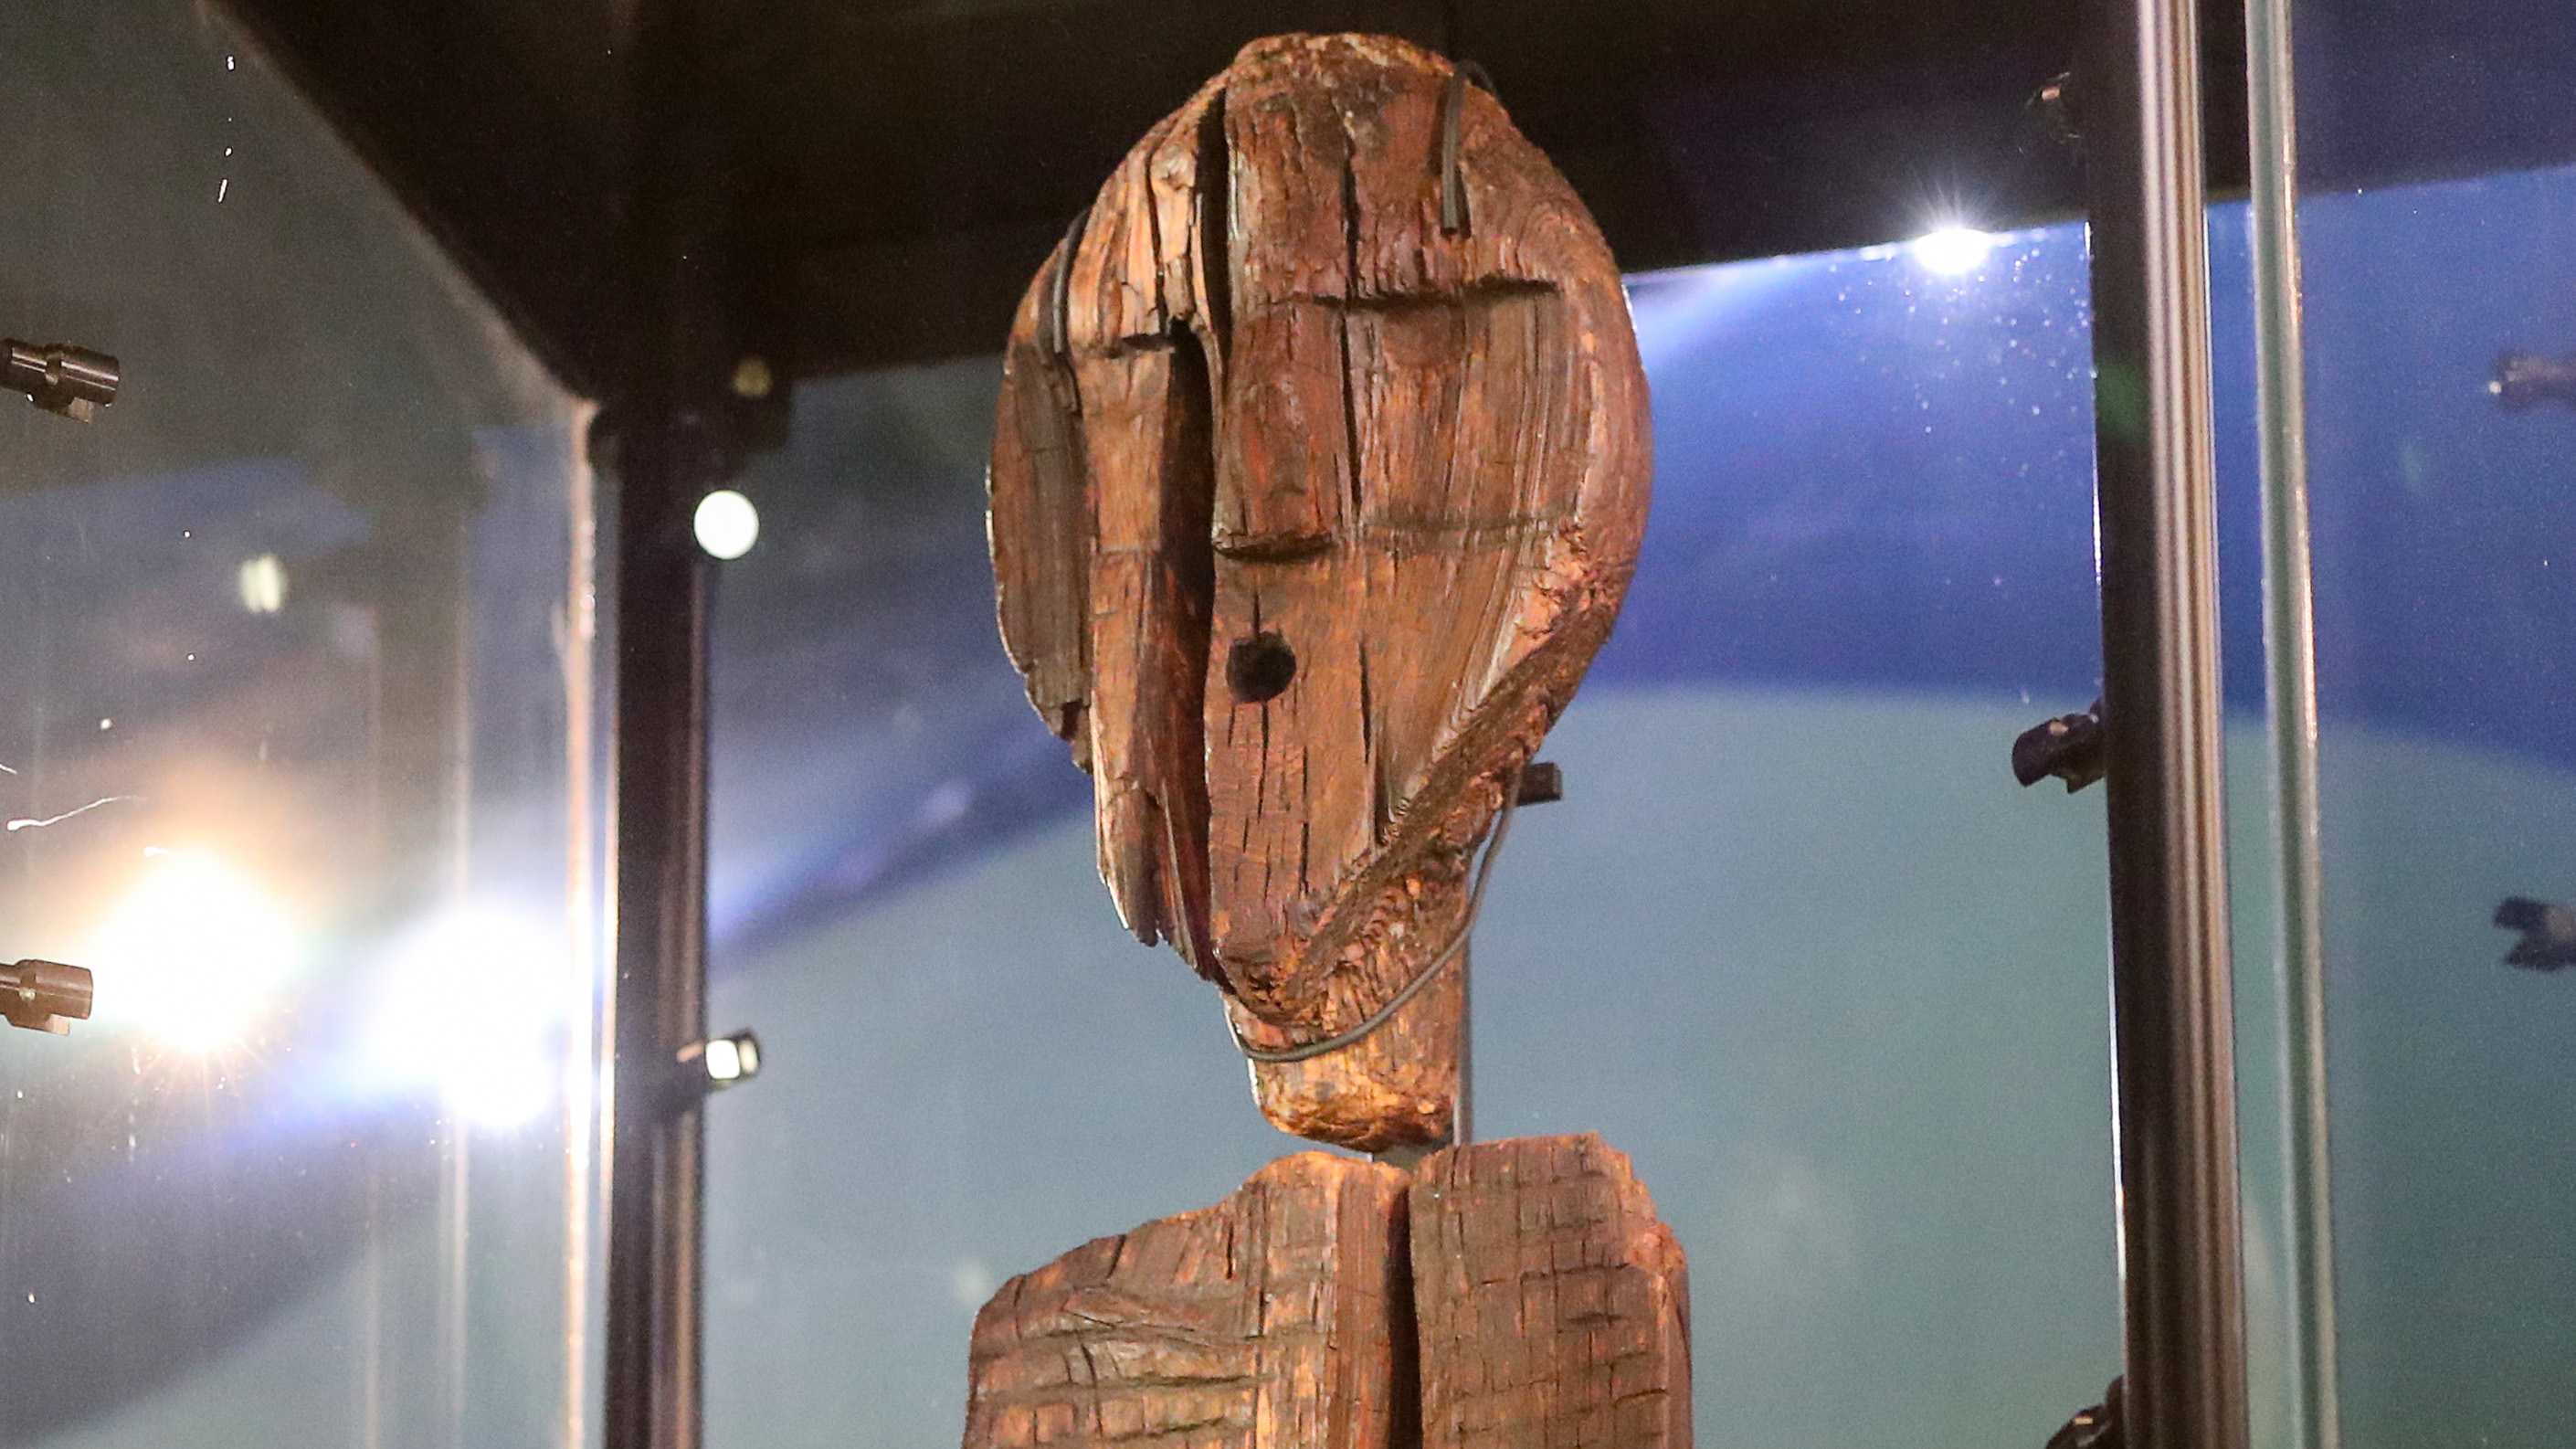
\includegraphics[height=4cm]{img/shigir}} {Source: \url{https://www.livescience.com/shigir-idol-older-than-thought.html}}
\caption{Shigir Idol}
\label{fig:shigir}
\end{figure}

Stone is one of the oldest sculptural materials. Stone sculptures are usually made of marble or sandstone, rarely granite or other types of stone. Sometimes they are made on the basis of a clay cast. The stone allows to show a given figure or object in three dimensions, emphasize individual facial features or details that the author of the sculpture wanted to emphasize. Among the most famous stone sculptures that have survived to modern times are Venus from Milo, as well as the Vatican Pieta and Michelangelo's David (\autoref{fig:stone-sculp}).

\begin{figure}[h]
\center
a) \copyrightbox{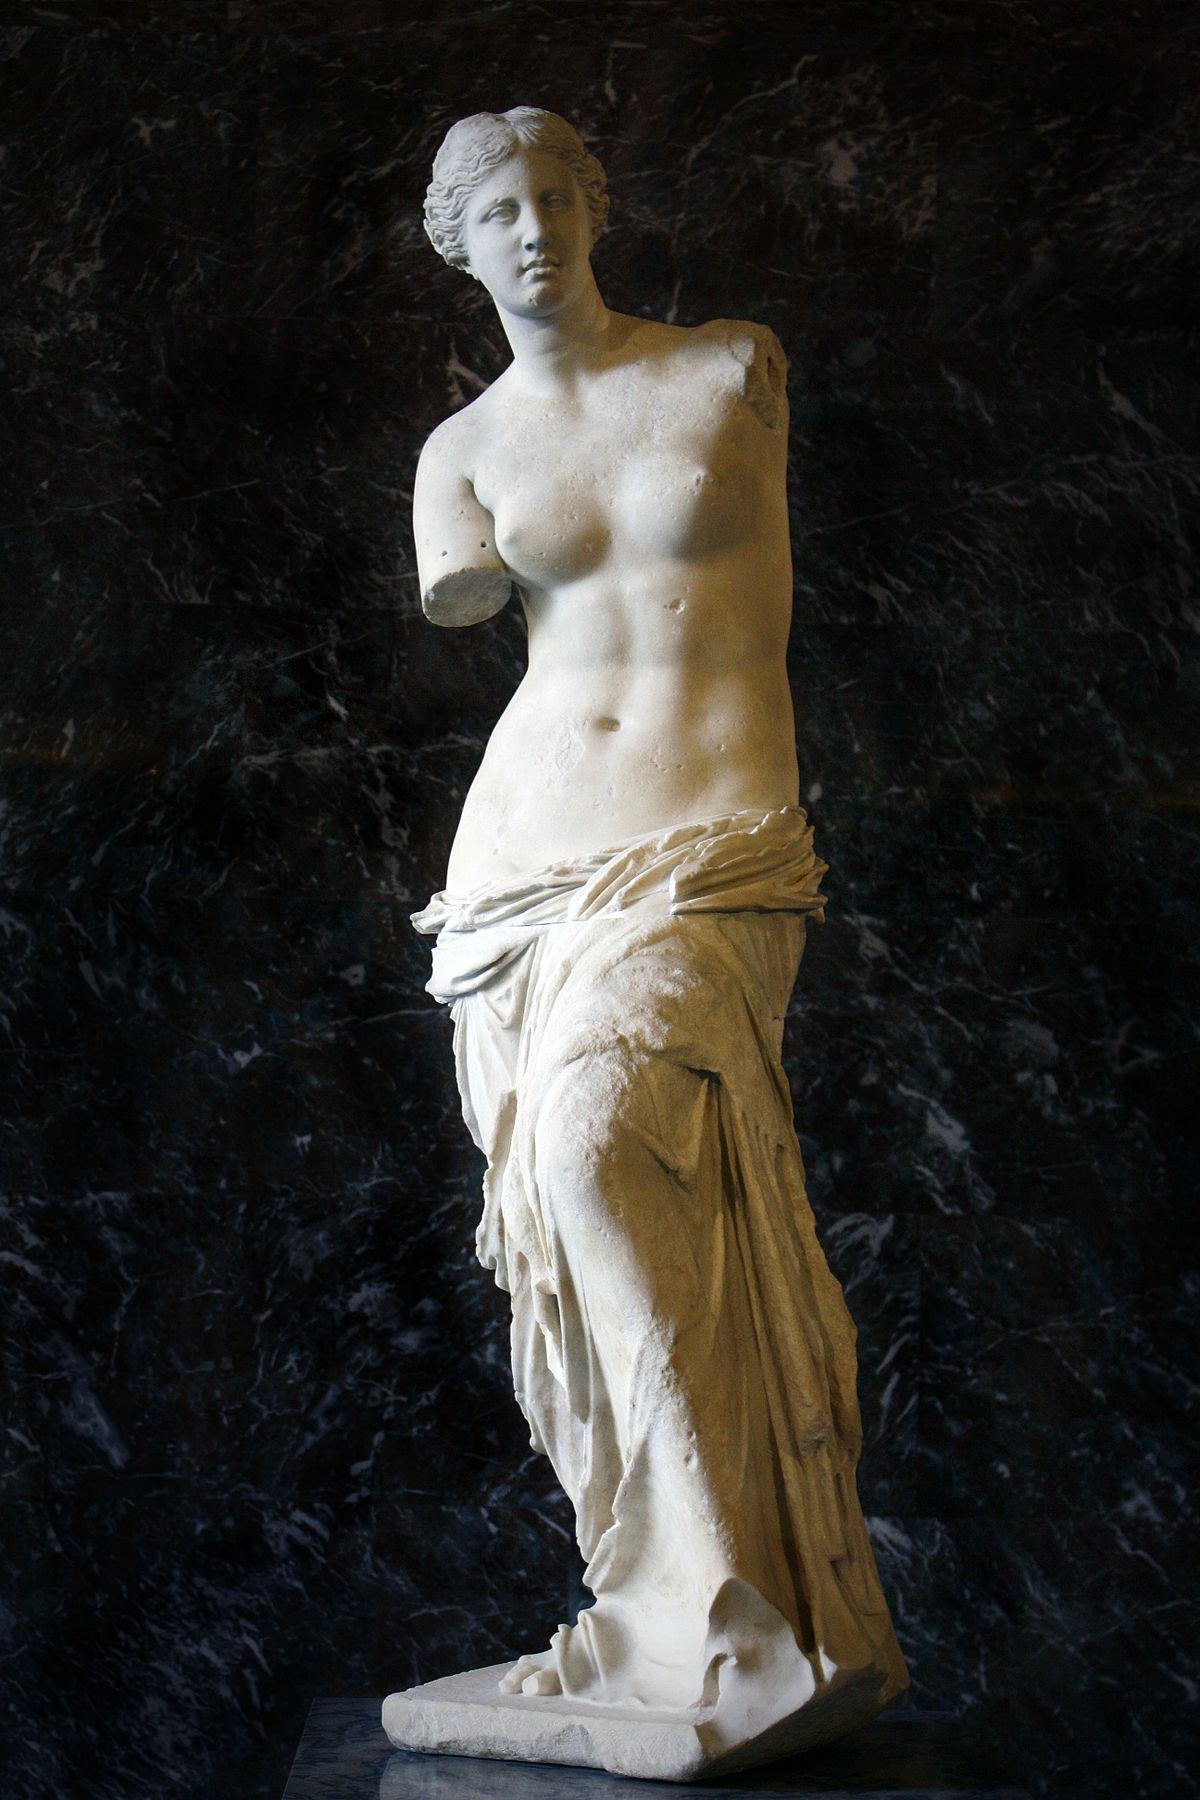
\includegraphics[height=3.5cm]{img/wenus}} {Source: \url{https://pl.wikipedia.org/wiki/Wenus_z_Milo}}
b) \copyrightbox{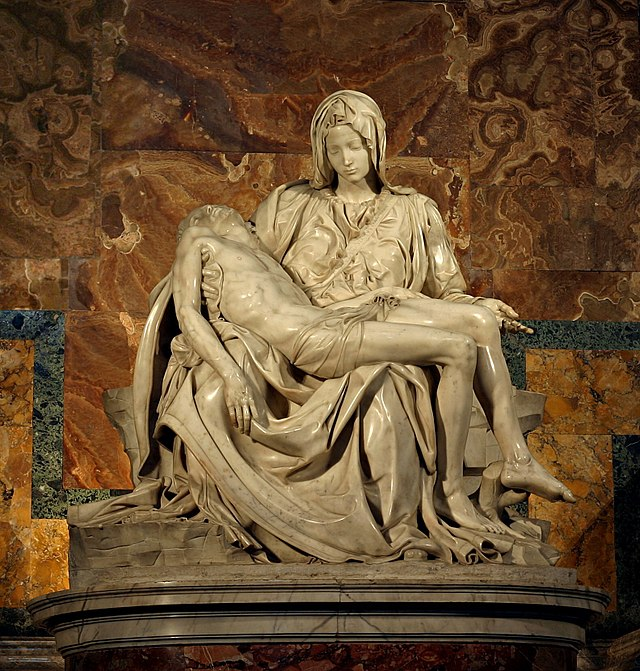
\includegraphics[height=3.5cm]{img/pieta}} {Source: \url{https://pt.wikipedia.org/wiki/Piet\%C3\%A0_\%28Michelangelo\%29}}
c) \copyrightbox{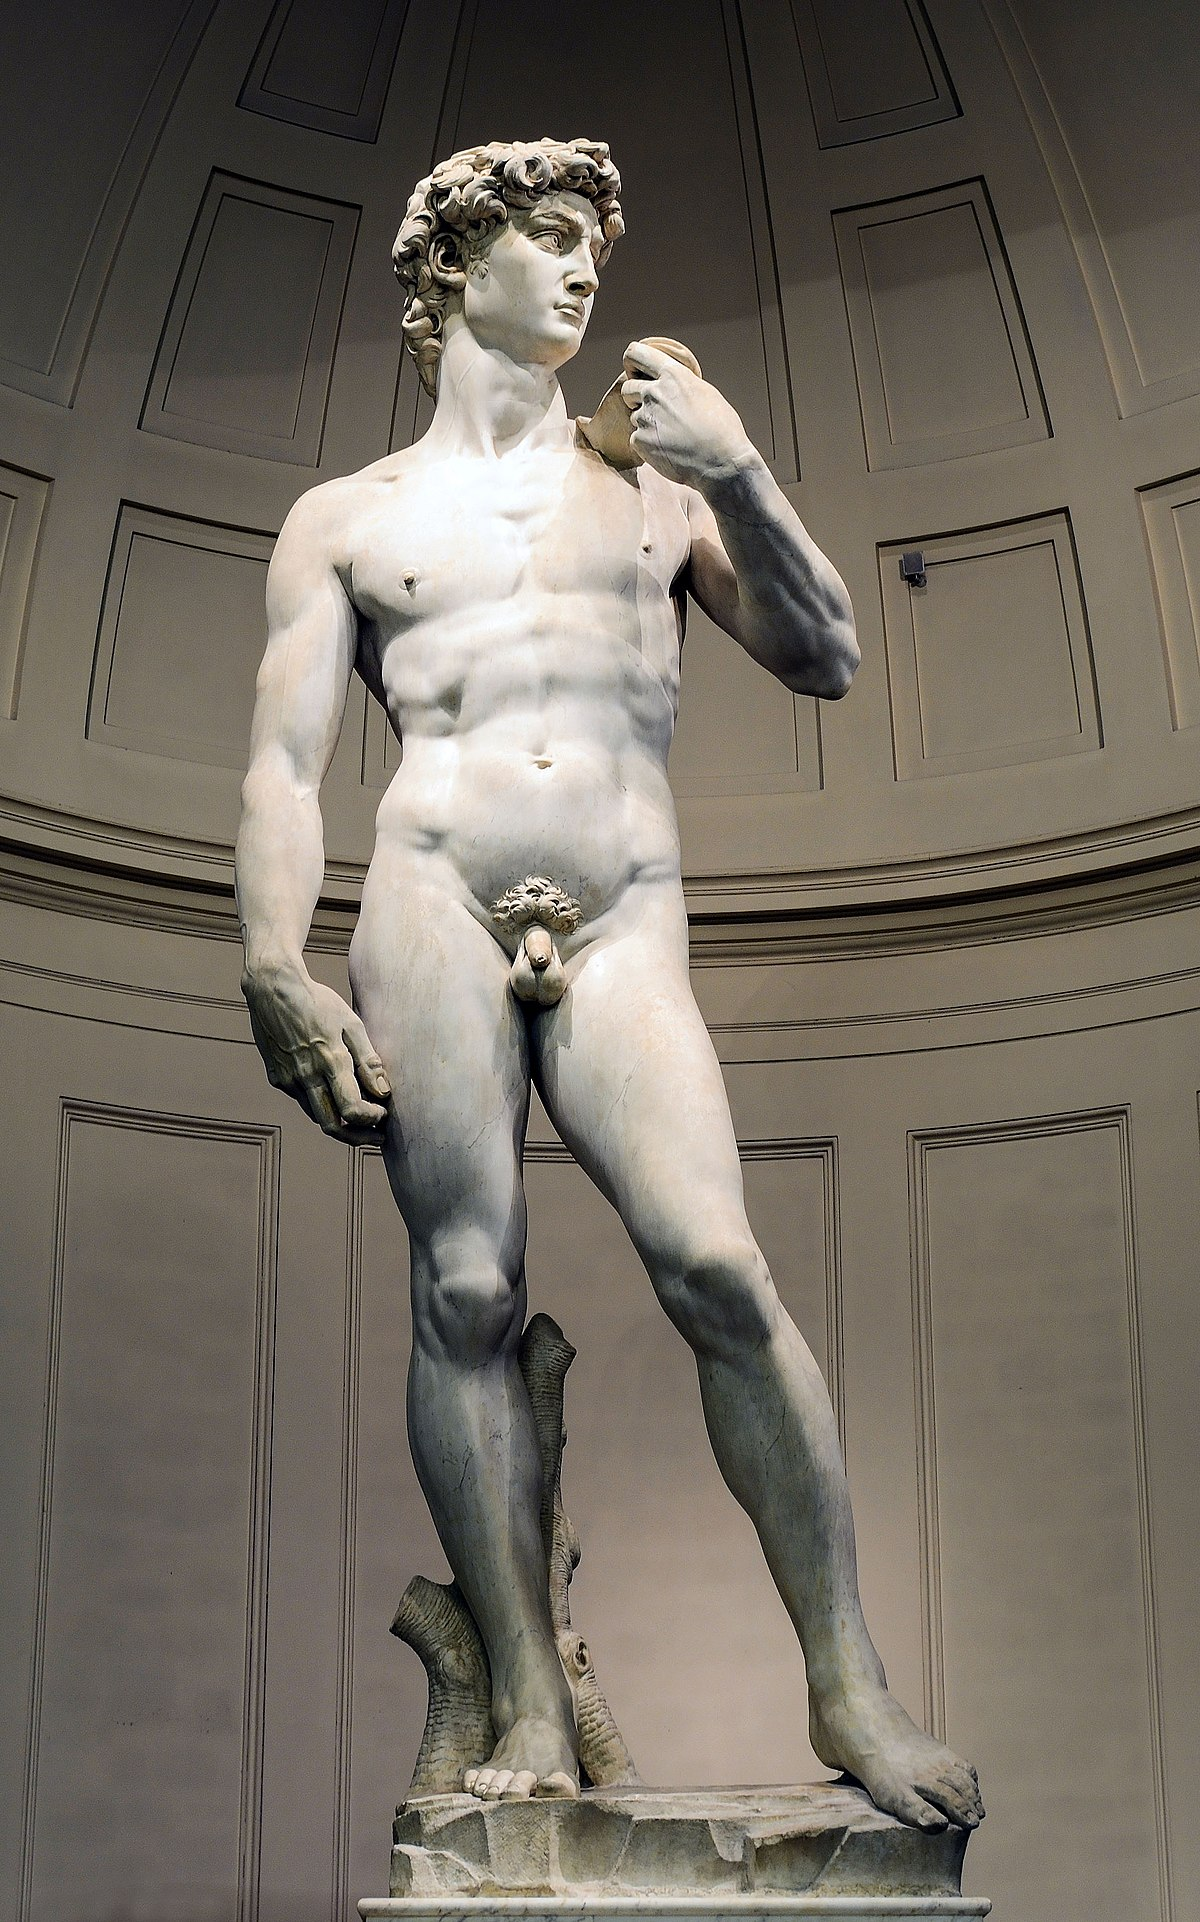
\includegraphics[height=3.5cm]{img/david}} {Source: \url{https://pt.wikipedia.org/wiki/David_\%28Michelangelo\%29}}
\caption{Famous stone sculptures: a) Venus from Milo,
b) Pieta, c) David}
\label{fig:stone-sculp}
\end{figure}


\section{Architecture}

Architecture is the science and art of designing, as well as constructing and then making various spatial structures. Architecture can also be called the totality of material objects that are the work of man and are permanently associated with a given area. These facilities are to meet the personal and social needs of a person. An element of architecture can be a sculpture placed in a park, a bench in a garden, a sidewalk, a house, a bridge, a road, an overpass and other objects of this type \cite{BOOK:5}.

Since antiquity, the goal set before the creators was that architectural objects affect people, hitting their sense of beauty, and the aesthetic elements of the created works have always been an important part of them. Over the centuries, styles prevailing in architecture have changed. Objects of exceptional artistic value are part of the cultural heritage and are considered masterpieces. Historical civilizations are often known mainly for their architectural achievements. Buildings such as the pyramids in Egypt and the Roman Coliseum (\autoref{fig:archi-symb}) are cultural symbols and are an important element of the nation's consciousness. Cities, regions and cultures are identified with architectural monuments.

\begin{figure}[h]
\center
a) \copyrightbox[b]{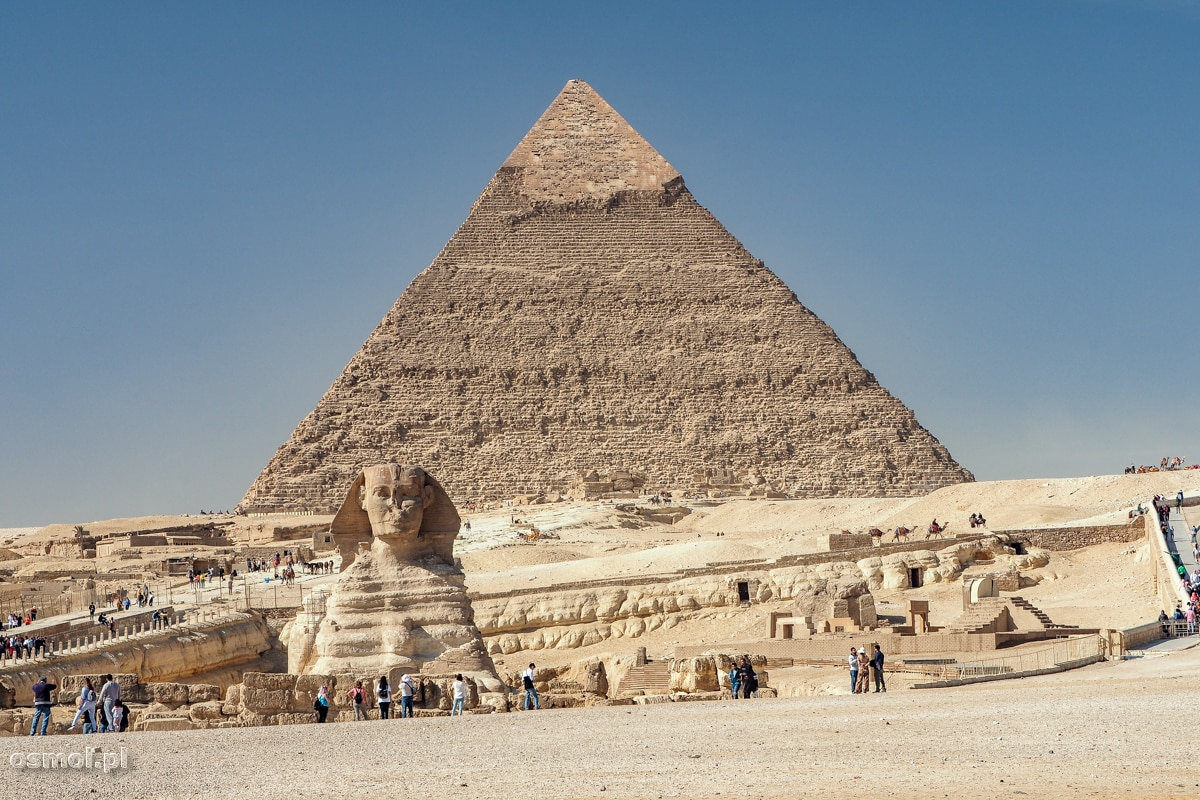
\includegraphics[width=5cm]{img/pyramid}} {Source: \url{https://www.osmol.pl/piramidy-w-gizie-egipt/}}
b) \copyrightbox[b]{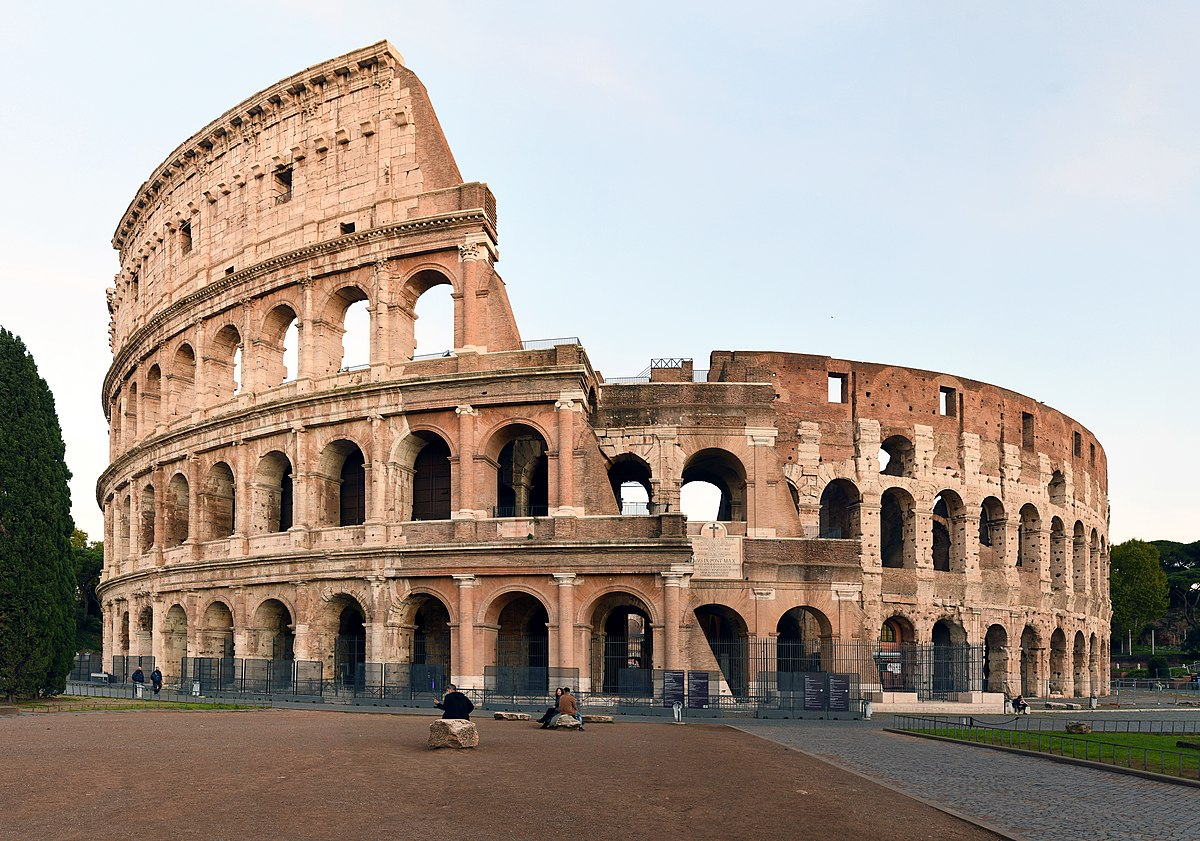
\includegraphics[width=5cm]{img/coliseum}} {Source: \url{https://pl.wikipedia.org/wiki/Koloseum}}
\caption{Examples of significant cultural architecture symbols: a) Pyramid in Giza,
b) Coliseum in Rome}
\label{fig:archi-symb}
\end{figure}


\section{Photography}
The art of photography is the art of creating realistic images by recording light on a surface, which faced a lot of development because of the industrial revolution and was constantly upgraded throughout the years.

In the year of 1825, Joseph Nicéphore Niépce created the first photography, unbroken until this day, called "View from the Window at Le Gras" (\autoref{fig:le-gras}).
The process to take photography, as mentioned earlier, was improved by chemists, physics and engineers throughout the years, they tested different chemicals to absorb the light and tried new materials to print the images. Glass was extensively during the 19th and 20th century, because of its accessibility. 

\begin{figure}[h]
\center
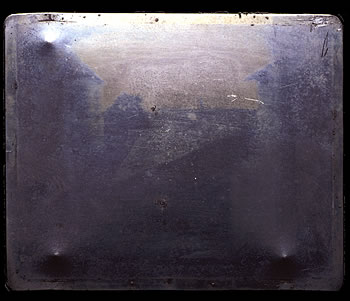
\includegraphics[width=5cm]{img/legras}
\caption{View from the Window at Le Gras by Joseph Niépce.}
\label{fig:le-gras}
\end{figure}

At the end of the 19th century, Gabriel Lippman created a process for natural-color photopgraphs and was awarded a Nobel Prize in Physics later in the 20th century for his invention.
In the 19th century, film was also invented by Louis Le Prince, although it was extremely expensive, it didn't gain as much popularity until the 50s.
After his invention, other techniques arose, like astrophography and laser holography.

In the year 1981, Sony created the first consumer camera MAVICA to extinguish the need of film, but the images were only displayable with a TV and Fujifilm unveiled a camera which both saved and recorded images on a semiconductor memory card - the FUJIX DS-1P - in 1988. It wasn't until 1991 when Kodak created the world's first fully digital camera - the DCS 100 (\autoref{fig:digital-cameras}). 

\begin{figure}[h]
\center
a) 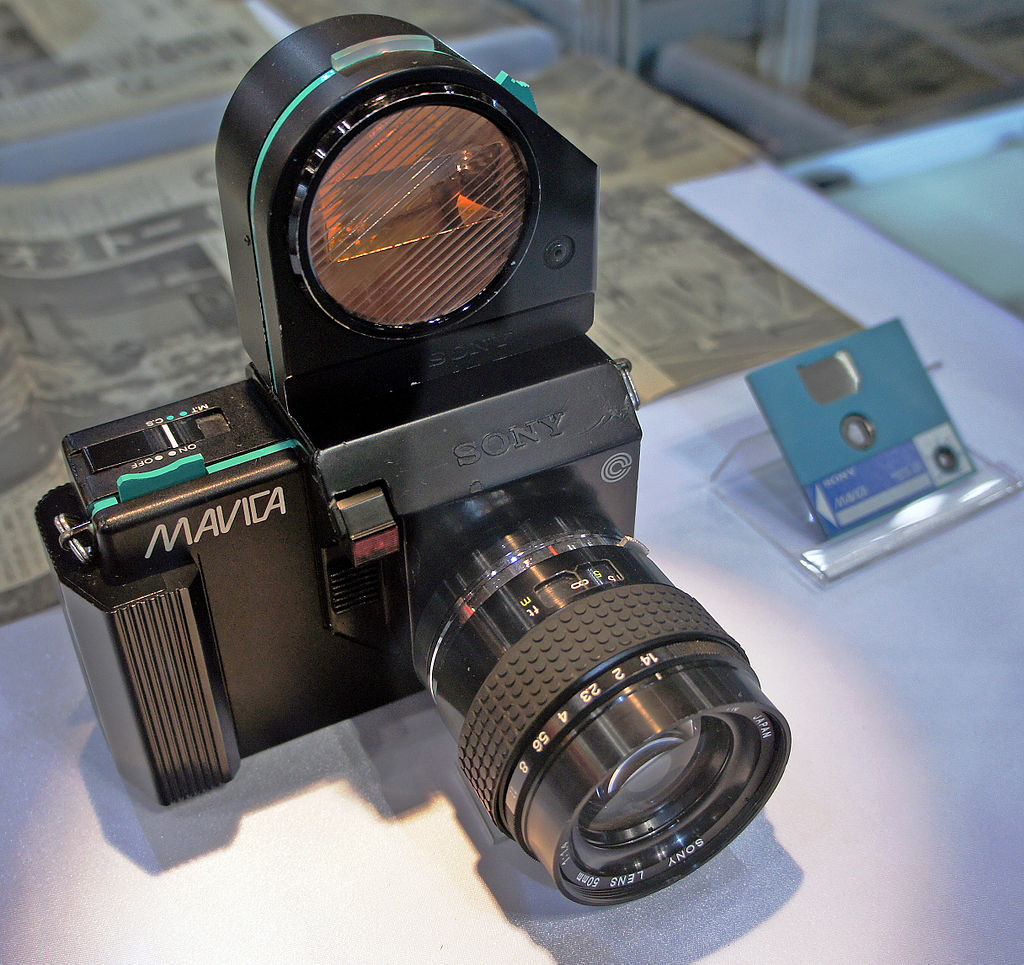
\includegraphics[width=5cm]{img/mavica}
b) 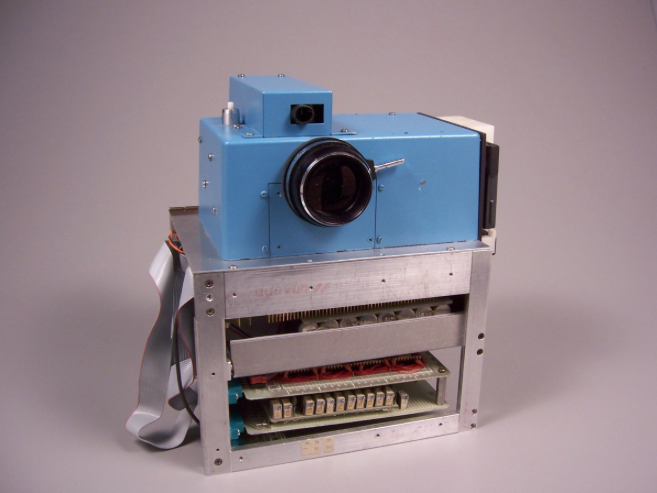
\includegraphics[width=5cm]{img/fujix}
c) 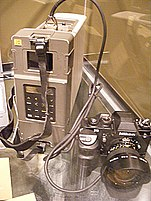
\includegraphics[width=5cm]{img/dcs100}
\caption{The most important digital cameras created: a) Sony MAVICA,
b) Fujifilm FUJIX DS-1P, c) Kodak DCS 100}
\label{fig:digital-cameras}
\end{figure}

This evolution enabled photography to be more accessible and leave its mark in society as a really important form of art and it also let regular sitizens use it for the sake of their social life, earn a living (like paparazzi, fashion photographers, advertisers), create art styles, like art photography, which was a technique tha tried to imitate paintings by using a soft and smooth focus, photojournalism, one of themost impactful styles of photography during times of war and wildlife photography, that had the objective of capturing the animal life for it's viewers.

\section{Music}
	
Music is a form of art that combines sounds, both vocal and instrumental, using the elements of melody, harmony, rhythm and timbre. It is present in all styles and art moviments during human history, it's culturally universal and present in all human societies. Today's music is the result of ongoing cultural evolution. Throughout it, music was and still is one of the most effective forms of art in terms of expressing emotion, being so impactful it can heavily influence human behavior.
	
As mentioned earlier, music can be found everywhere. It's history consists on a variety of its adjunctive function in rituals and ceremonies, like regilious, military, courtly, etc. Music's flexibility allows itself to bond easily with literature, dance and drama.

Listening to music for the sake of enjoying it, unrelated to ritauls or storytelling,  is a noticeably a new thing in our history. 
Music in the past has been mostly enjoyed by upper-class citizens, existing barely any public theaters or opera houses until the 18th century. Nowadays, there's a far-reaching group of genres of music, most popularly: pop music, rap, hip-hop, rock and eletronic. Pop culture specially has brought music to peoples lives by introducing it with radio, film, TV, musical theatres and the internet. As technology evolved, these possibilities became intrinsic to us. Music is also sometimes used in the medical field to improve conditions such as:
\begin{itemize}
 \item{Conditions related to cardiac problems;}
 \item{Depression;}
 \item{Autism;}
 \item{Substance abuse;}
 \item{Alzheimer.}
\end{itemize}
And it can help improve:
\begin{itemize}
 \item{Coping;}
 \item{Reduce stress;}
 \item{Improve self-esteem;}
 \item{Etc.}
\end{itemize}

\chapter{Most Influential Art Movements}
\label{chap.influential_art_movements}

\section{Cubism}

Cubism is one of the trends in the visual arts, primarily related to painting and sculpture, which had its beginning in France around 1907. Its founders focused mainly on the search for completely new principles of the spatial construction of a work by completely rejecting the known rules of perspective. In addition, the representatives of cubism wanted a strong, even geometrical simplification of the elements of the entire composition, which was clearly noticeable in each work. 

A characteristic feature of cubism is primarily a narrow thematic circle, as the most common motives include still life, portraits and landscapes. In addition, this trend is characterized by a modest color palette, limited mainly to browns, greens and grays. The paintings usually show an object seen from many sides, which is called simultaneousism, because the artists assumed that the recipients of their works would be intelligent enough to put the presented thing together. For this reason, it can be said that the cubists believed that painting results from the knowledge of the object, and not from seeing it directly. The effect of the cubists' activities was to show a multiplied space with a clear structure, which is why their works cannot be classified as fully abstract \cite{BOOK:2}.\medskip

Some examples of leading artworks:
    \begin{itemize}
    \item{Pablo Picasso's "Les Demoiselles d'Avignon" (\autoref{fig:avignon})}

An artwork depicting five naked women. Two of them are more clearly illuminated and isolated from the background. The other three women, on the other hand, are presented in an unrealistic way, and the main deformation concerns their faces. There is no perspective in this painting, because both the figures and the background are one whole. The colors are mild for the eye. It is a cubist painting in which one can notice the geometrisation of female silhouettes and the body broken into several individual fragments.

\begin{figure}[h]
\center
\copyrightbox[b]{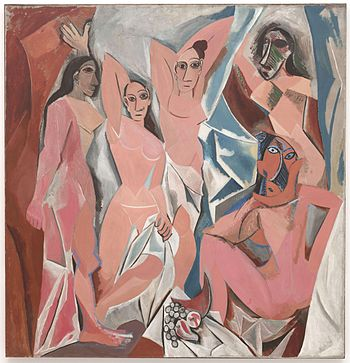
\includegraphics[height=7cm]{img/picasso-1}} {Source: \url{https://en.wikipedia.org/wiki/Les_Demoiselles_d\%27Avignon}}
\caption{Pablo Picasso's "Les Demoiselles d'Avignon"}
\label{fig:avignon}
\end{figure}

    \item{Pablo Picasso "Guernica" (\autoref{fig:guernica})}
    
A cubist painting that is an act of protest against violence and at the same time a manifestation of pacifism, thanks to which it has a clear message. The work shows deformed human and animal figures that form one chaotic whole. Fragments of limbs, bodies and heads are visible, and the mouth is usually open in a silent scream. There is obvious terror in her eyes. The image is full of dynamics and maintained in monochromatic colors.

\begin{figure}[h]
\center
\copyrightbox[b]{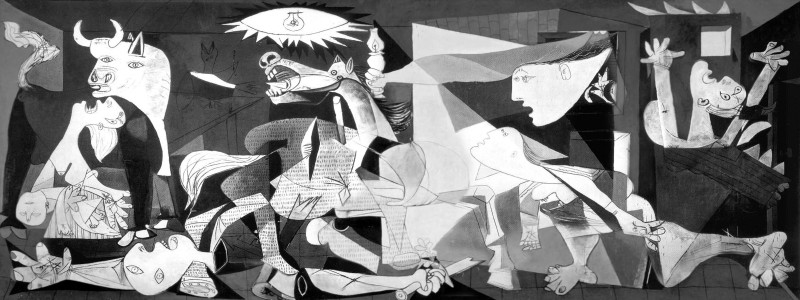
\includegraphics[height=4cm]{img/picasso-2}} {Source: \url{https://www.infoescola.com/pintura/guernica/}}
\caption{Pablo Picasso  "Guernica"}
\label{fig:guernica}
\end{figure}

    \end{itemize}

\section{Renaissance}

The Renaissance is a period in human history (between the 14th and early 17th century) when western Europe had to revive itself (as the name renaissance suggests, renaissance means rebirth in english) from a crushing instability after hundreds of years of strenght, caused by political, religious and demographic collapse.	It's the transition between the middle ages and the modern world and it generated extraordinary social change... And lots of art. During this period, it emerged developments on the social status of men and woman, the importance of understanding and learning philosophy, literature, technology and science.	It was also created an outlook on religion by the people because of the greater understanding of science and the questioning by philosophy. 

Some of the most known art pieces are:

\begin{itemize}
    \item{Leonardo da Vinci's "Mona Lisa" (\autoref{fig:monalisa})}
    
Mona Lisa is today's most popular and expensive painting. The art piece, made by da Vinci in 1503, resembles a portrait of a Lisa del Giocondo, a noblewoman married at the time to the wealthy Florentine silk merchant Francesco del Giocondo. The painting bears semblance to Virgin Mary, which was at the time viewed as the ideal woman. Da Vinci used various techniques common during the Renaissance period, like aerial prespective and it affects the light based on the distance between the viewer and the object. As we can observe, the contrast of the background decreases, giving the impression that it's quite blurry. Another technique also used by Leonardo in Mona Lisa is sfumato, which makes the transition between colors incredibly smooth and gives an elusive rendering of her Lisa's face. Da Vinci himself described this technique as painting without lines, "in the manner of smoke".
	    
\begin{figure}[h]
\center
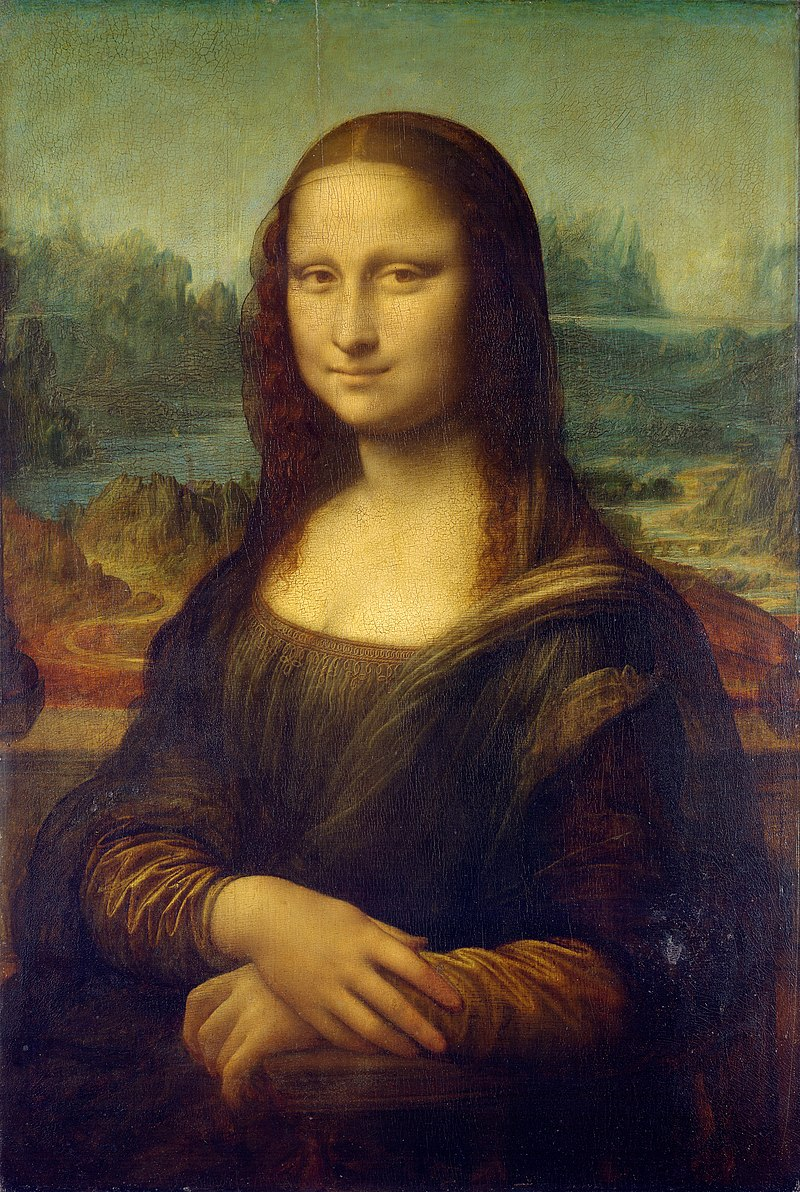
\includegraphics[height=4.5cm]{img/monalisa}
\caption{Leonardo da Vinci's  "Mona Lisa"}
\label{fig:monalisa}
\end{figure}

	\item{Raffaello da Urbino's "School of Athens" (\autoref{fig:schoolofathens})}

Raffaello's "School of Athens" pictures a group of various polymaths, philosophers, mathematicias, scientists, engineers and artists. It includes Plato, Aristotle, Pythagoras, Archimedes, Heraclitus, Leonardo da Vinci and Michelangelo, between others. The painting tries to describe to the viewer the true embodiement of the Renaissance, and the hunger for knowledge during the period. Raffaello's put Leonardo in the center of the painting, counting as a nice gesture since he learned how to paint with prestective from him. 
		    
\begin{figure}[h]
\center
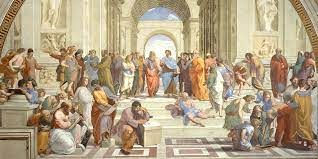
\includegraphics[height=5.3cm]{img/schoolofathens}
\caption{Raffaello da Urbino's "School of Athens"}
\label{fig:schoolofathens}
\end{figure}

\end{itemize}
    
\section{Surrealism}

Surrealism originated in France in 1924. The period in which he was born was called the age of dreams. Surrealism in painting assumed the visual expression of internal perception. Artists created images that contradicted the logical order of reality. They seemed grotesque and dreamlike. They negated the assumptions of realism, classicism, empiricism, utilitarianism and rationalism. Surrealism externalized dreams, subconscious states, and associated all elements completely randomly. This trend drew its inspiration from dadaism.

\begin{figure}[h]
\center
\copyrightbox[b]{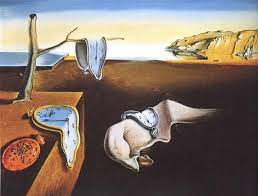
\includegraphics[height=6cm]{img/dali}} {Source: \url{https://www.wikiart.org/en/salvador-dali/the-persistence-of-memory-1931}}
\caption{Salvador Dali "The Persistence of Memory" -  example od surrealistic painting}
\label{fig:dali}
\end{figure}

Surrealist painters presented irrational visions influenced by free associations. They did not limit their imagination and created without any inhibitions. They rebelled against moral norms, social rules and any order. They wanted to provoke and create absurd images. In the center of their interest were primarily the possibilities of the human mind. Surrealists were fascinated by automatic writing, hypnosis, mediumism for example phenomena that were studied by psychoanalysis at that time \cite{BOOK:2}. They found wonder in ordinary things and dramatized seemingly trivial events. The element of surprise, nonsense and absurdity was of great importance to them.\medskip

The representatives of surrealism include, among others:
\begin{itemize}
 \item{Salvador Dali}
 \item{Max Ernst}
 \item{Hans Arp}
 \item{Joan Miro}
\end{itemize}


\section{Impressionism}

The impressionists were fighters for freedom in art, and impressionism itself was its revolution. The strand that initiated impressionist painting was completely different from realism, which reigned in the art world not long before. For the creators of this trend, the world as it is did not matter. The Impressionists did not want to imitate reality, but to impose on it a filter of sensations that they or the heroes of their works felt at a given moment \cite{BOOK:3}.

The features of impressionist painting are primarily efficient manipulation of light and shadow. Impressionist artists blurred the line between reality and fiction, creating something in between - a transition between worlds. It was the two elements of impressionism - shadow and light - that gave the paintings an unreal dimension. They were supposed to change colors, sharpen or blur contours, give dynamics to things, characters and landscapes. The characteristics of impressionism were clearly shown by Pierre Auguste Renoir in the painting "The Ball at the Moulin de La Galette" (\autoref{fig:moulin}). In addition to playing with light, Renoir also used another feature of impressionism in art - inspiration from urban life. This city itself as a living organism that is constantly in motion, changing, being the center of life of its inhabitants, created a typical impressionistic landscape.

\begin{figure}[h]
\center
\copyrightbox[b]{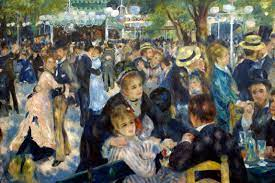
\includegraphics[height=5.7cm]{img/moulin}} {Source: \url{http://www.codex99.com/unclassified/moulin-de-la-galette.html}}
\caption{Pierre Auguste Renoir "The Ball at the Moulin de La Galette"}
\label{fig:moulin}
\end{figure}

The impressionists adored dynamics, and in everyday life it was best reflected in social life. Many impressionist paintings were dedicated to the theme of dynamic trysts, colorful balls or the bustle of bars and taverns. An example may be the famous "Luncheon of the Boating Party" (\autoref{fig:boat-party}) by one of the leading representatives of impressionism, Pierre Auguste Renoir. Looking at the painting, it is difficult to clearly state whether the artist was an observer or a participant in the banquet \cite{BOOK:4}.

\begin{figure}[h]
\center
\copyrightbox[b]{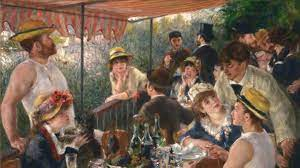
\includegraphics[height=5.7cm]{img/renoir}} {Source: \url{https://en.wikipedia.org/wiki/Luncheon_of_the_Boating_Party}}
\caption{Pierre Auguste Renoir "Luncheon of the Boating Party"}
\label{fig:boat-party}
\end{figure}

The impressionists did not abandon nature in favor of man, a good example of which is Claude Monet's "Water Lilies" from that period. An important element of the work of this period were also impressionist landscapes. This is “Impression. Sunrise” by Monet gave the name to this art direction (\autoref{fig:monet}).

\begin{figure}[h]
\center
a) \copyrightbox{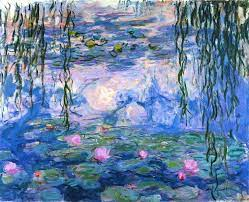
\includegraphics[height=3.3cm]{img/lilies}} {Source: \url{https://www.wikiart.org/en/claude-monet/water-lilies-1919-1}}
b) \copyrightbox{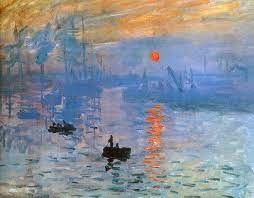
\includegraphics[height=3.3cm]{img/sunrise}} {Source: \url{https://en.wikipedia.org/wiki/Impression,_Sunrise}}
\caption{Examples of impressionist landscapes: a) Claude Monet "Water Lilies",
b) Claude Monet “Impression. Sunrise”}
\label{fig:monet}
\end{figure}

\section{Expressionism}

The word "expressionism" comes from Latin and means "expression". This direction in art developed in Germany in the first 30 years of the 20th century. It was a form of opposition to the naturalistic attitude. Expressionism in art was created by the generation born between 1875 and 1895. Its greatest flourishing and activity could be observed in the years 1910-1925 \cite{BOOK:2}.

\begin{figure}[h]
\center
\copyrightbox[b]{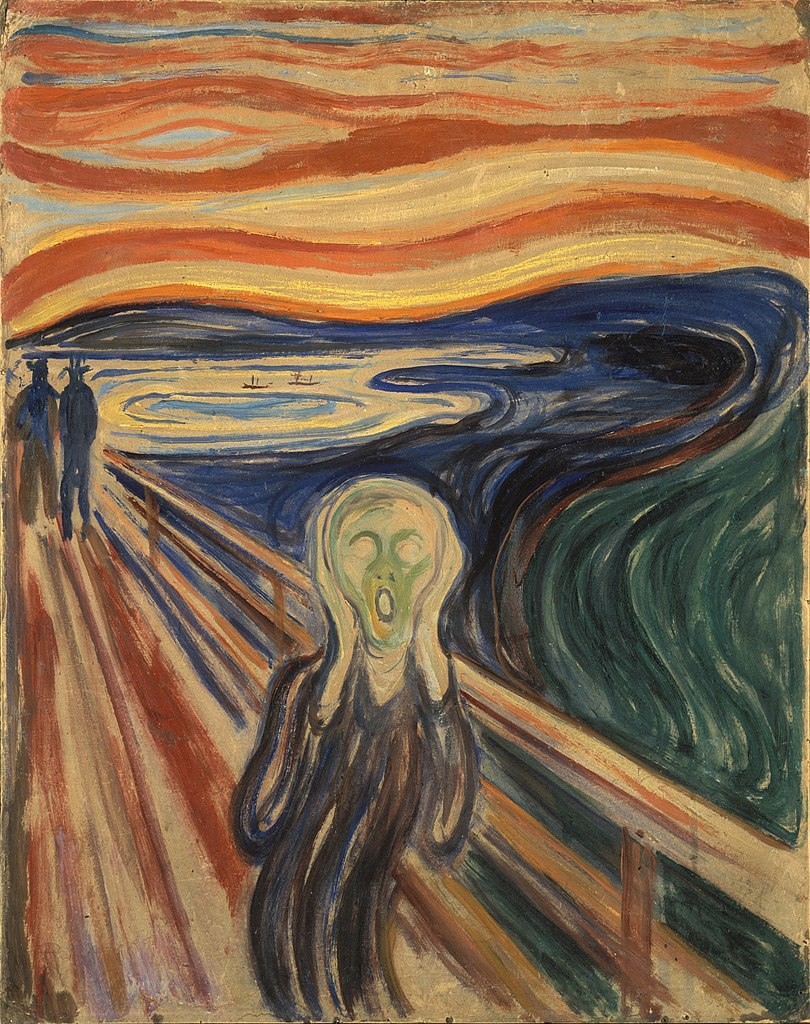
\includegraphics[height=6cm]{img/scream}} {Source: \url{https://smarthistory.org/munch-the-scream/}}
\caption{Edward Munch "The Scream" - example of expressionism style}
\label{fig:scream}
\end{figure}

This direction in painting was characterized by deformation and sharply painted outlines of objects. The creators and followers of expressionism were terrified of the emptiness and barrenness of modern life. They opposed the ubiquitous primitivism and materialistic approach to life. In addition, the artists feared that the developing technology and mechanization would threaten human freedom \cite{BOOK:2}. Expressionism was about expressing the artist's feelings. This direction in art rebelled against naturalism and the bourgeois approach to life. Expressionists believed that the purpose of art is to create an image of the inner world of man. The task of art was to recreate one's own inner experiences, to express spiritual tensions, such as anxiety or terror.

The most outstanding representative of the expressionist work is the painting "The Scream" (\autoref{fig:scream}) by the Norwegian artist Edward Munch. Painted in 1893, it was almost immediately hailed by critics as Munch's greatest work. Against the background of a distorted image, the painter, using bold colors (various shades of red - from orange to yellow), showed a screaming figure to depict human nature. The effect of terror, mystery and danger was intensified by the use of wavy lines and painting two unidentified figures on the bridge.



\chapter{Modern Art Movements}
\label{chap.modern_art_movements}

\section{Street Art}

Street art, as the name suggests, is an art created on the street and in open spaces. The term includes graffities and murals, but also any sculptures, stickers, posters, video projections and art installations that are not confined by any building. Street art has no set rules, everyone creates according to their own rules, using the methods they want to create. The tradition of the trend is impermanent, illegal works are often removed by cleaning services. Recently, more and more often, the authorities take the initiative and employ artists.\medskip

Forms of Street Art:
    \begin{itemize}
    \item{Mural}
    
\begin{figure}[h]
\center
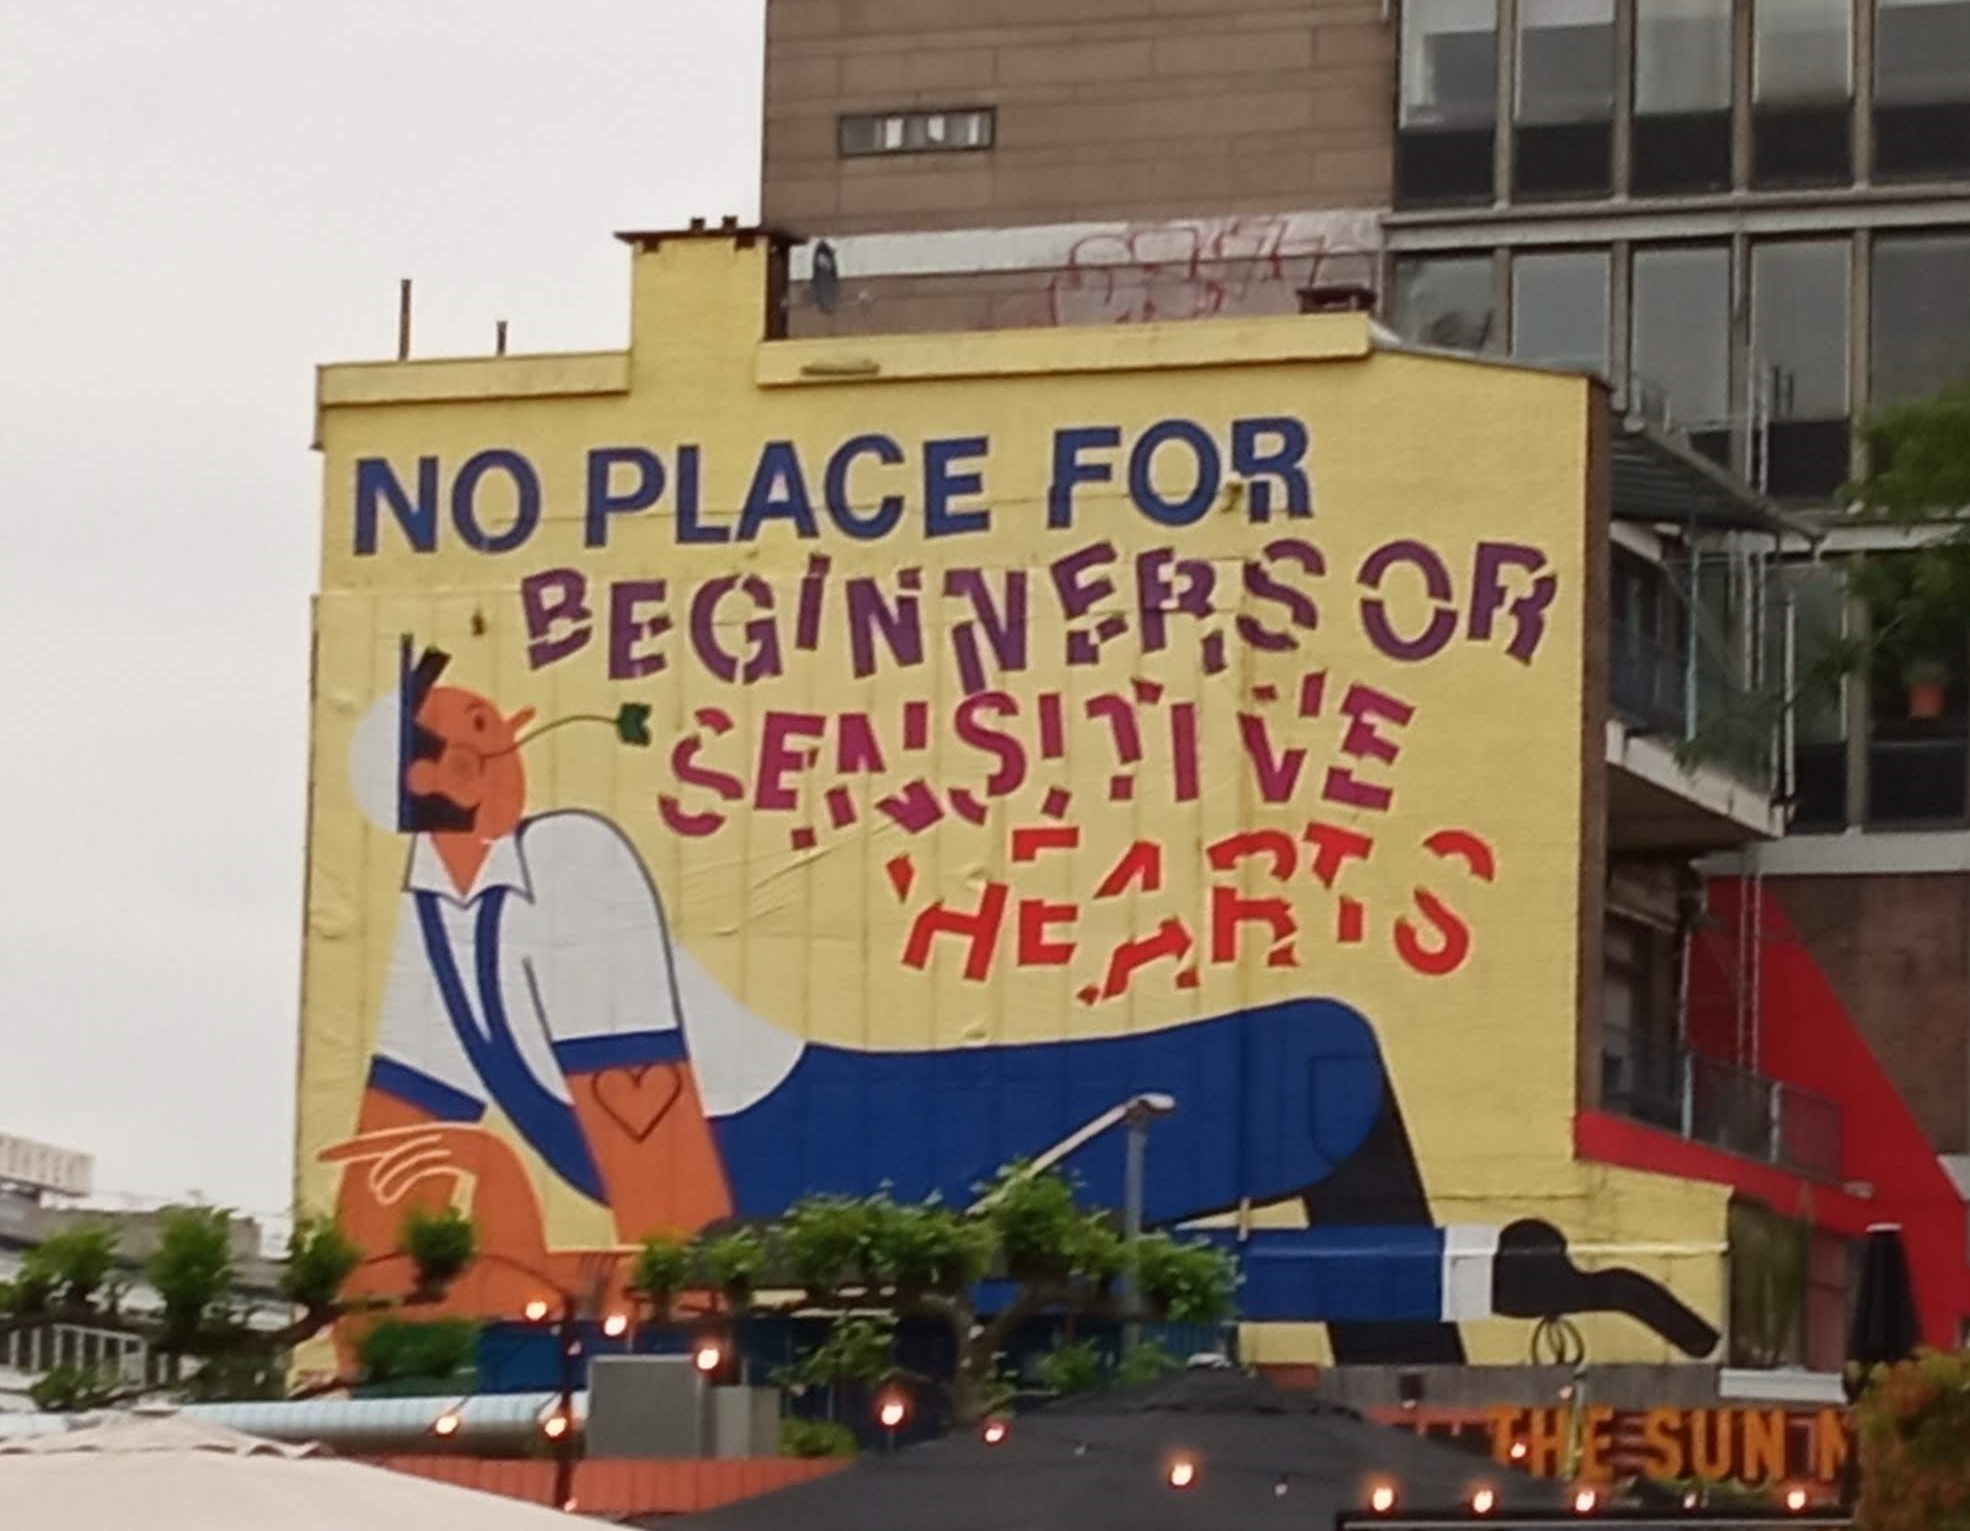
\includegraphics[height=6cm]{img/mural}
\caption{Example of mural found in Rotterdam}
\label{fig:mural}
\end{figure}
    
    A word coming from Spanish and meaning a large-scale painting painted on the wall for decorative purposes. The term most often used to refer to large-format paintings that are created on the walls of buildings. Murals are planned and carefully executed on walls, sometimes even with the help of scaffolding.
   
    
    
    \item{Graffiti}
    
    This term describes the textual forms of street art , most often done with a spray or brush. The images only serve as a background or padding. Often the style of writing letters is so elaborate that reading the inscription could be a problem. A characteristic feature is making images in a hurry, which results in little attention to detail. Initially, the authors made their inscriptions only in illegal places, without having time to work out the details.
    
    \item{Sticker}
    
    Small form of street art, which is somewhere on the border of advertising and art. Stickers most often appear in large clusters on advertising poles, municipal electrical boxes, gutters or in buses. They usually have a single idea to communicate. They can be a form of advertising for street artists, contain their pseudonym or Instagram account name or they can be just a simple drawing with a funny slogan. They make an interesting impression when they are in large groups.
    
    \begin{figure}[h]
\center
a) 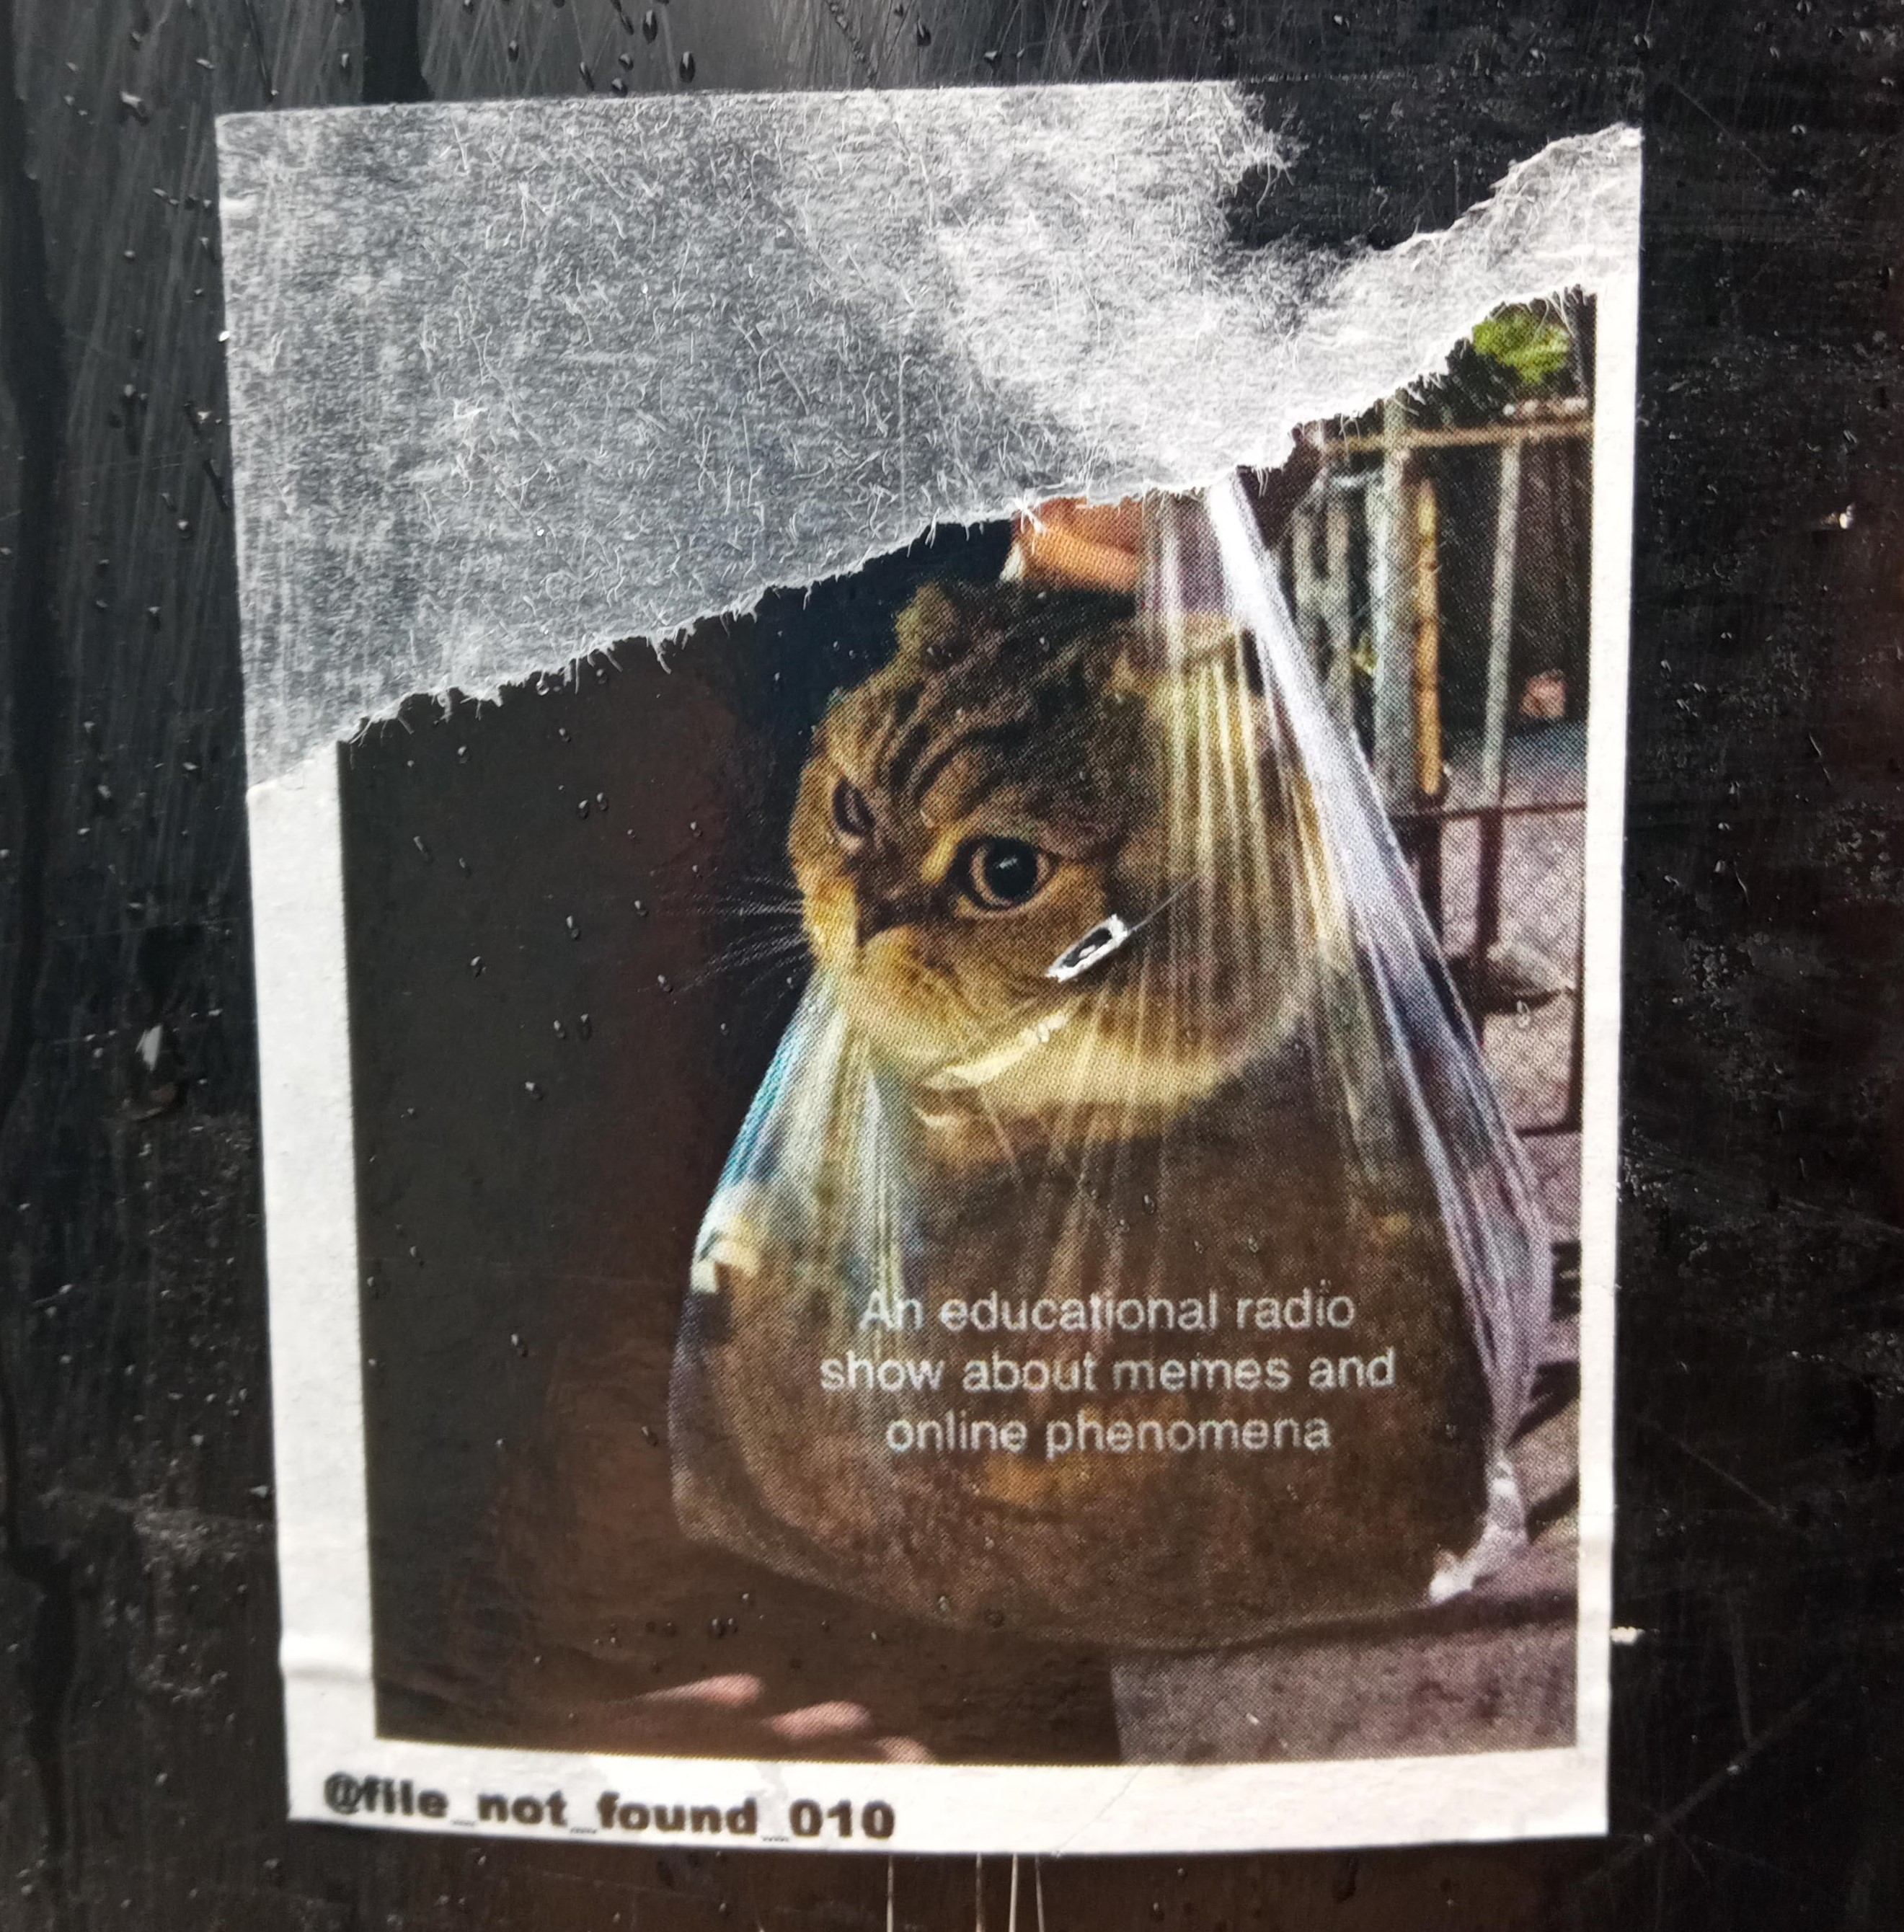
\includegraphics[height=6cm]{img/sticker}
b) 
\includegraphics[height=6cm]{img/stickersGroup}
\caption{Examples of stickers: a) Single sticker on electrical pool in Rotterdam,
b) Group of stickers on Lennon's Wall in Prague}
\label{fig:stickers}
\end{figure}
  

	\item{Tag}
     
     Graffiti artist's signature on the wall. Usually done very quickly, without any additional frills and details. It is the simplest form of graffiti. There is also peculiar type of tags known as "moving tag", which means a signature made on the train.
    \end{itemize}
    
    \medskip
The main Street Art creators:
    \begin{itemize}
    \item{TAKI 183}
    
	One of the first and most recognizable taggers was TAKI 183 (\autoref{fig:taki-183}). The artist worked as a courier, delivering parcels by subway, tagging the city. He became famous for having the most tags in all of New York at one point in his "career" \cite{WEBSITE:1}.
	
	\begin{figure}[h]
\center
\copyrightbox[b]{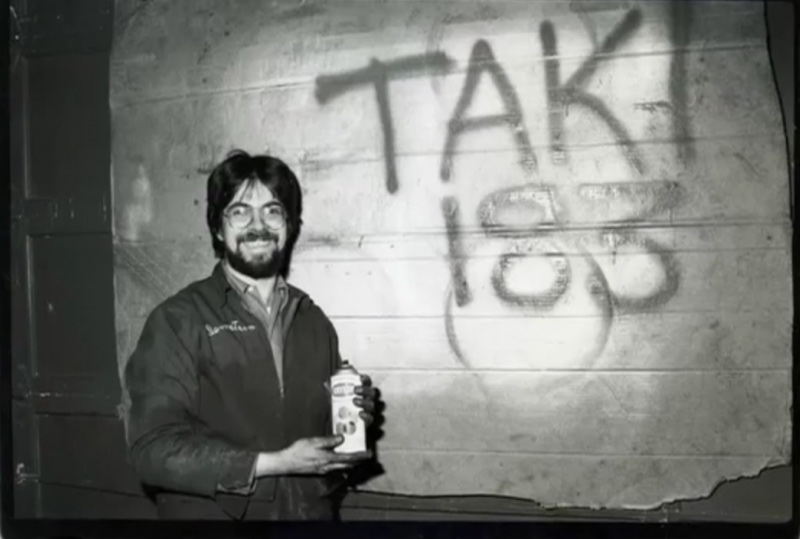
\includegraphics[height=6cm]{img/taki-183}} {Source: \url{https://urbanario.es/preguntas-sobre-el-graffiti-fue-taki-183-realmente-el-primer-grafitero/}}
\caption{Photo of TAKI 183 with his tag}
\label{fig:taki-183}
\end{figure}
    
    
    \item{Banksy}
    
	Artistic pseudonym of the creator of world-famous murals. His real name and face are shrouded in mystery. His murals are a combination of graffiti and stencil painting. He deliberately creates his works in such a way as to confuse the audience (\autoref{fig:banksy}). Street art in his performance forces to think, and accidental places of implementation mean that it is possible to come across them unexpectedly in different places around the world \cite{WEBSITE:1}.
	
	\begin{figure}[h]
\center
\copyrightbox[b]{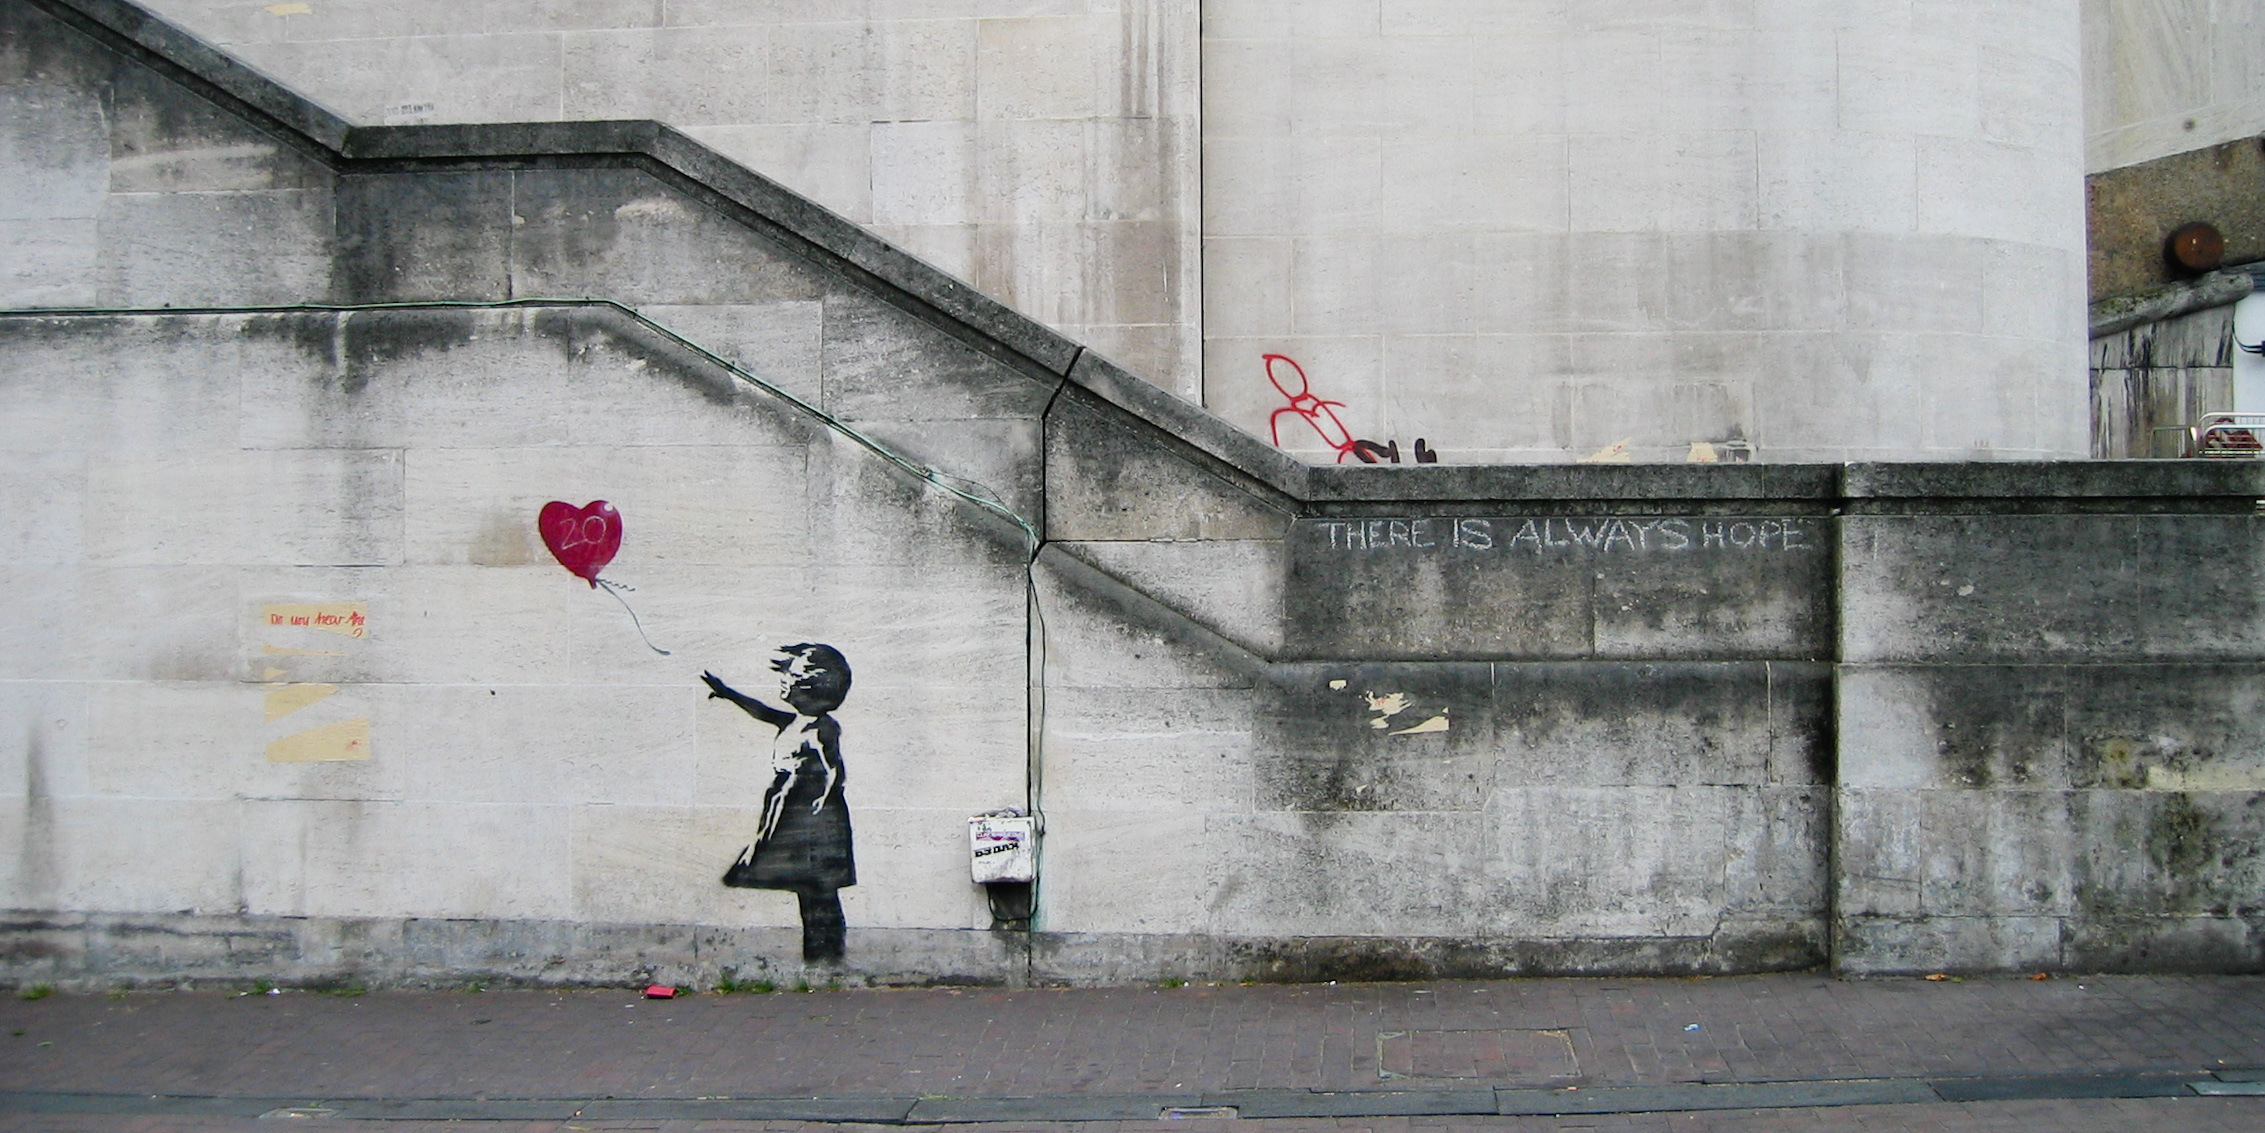
\includegraphics[height=6cm]{img/banksy}} {Source: \url{https://en.wikipedia.org/wiki/Girl_with_Balloon}}
\caption{Banksy "Girl with Balloon"}
\label{fig:banksy}
\end{figure}	
	
    \end{itemize}
    





\section{Digital Art}
\label{sec.digital.art}

The digital art era started in 1960, after technology made it's way into artists lives. For art to be considered digital, it has to be done using digital technology as it's fundation as a creative process. Digital paintings that are made in a traditional way are very common and artists nowadays usually commission for this style. Any software to make traditional digital paintings provides the artists with different brushes, styles, techniques and much more to their liking. There's a handful of privileges for choosing digital art, it's easier to make corrections, preparation and tracing, the supplies are free and so are many softwares

Examples of digital artwork are:
	\begin{itemize}
	\item{Traditional digital painting} (\autoref{fig:traditionalart})
	
In this image we can see an example of a traditional art, aswell as a software used by today's artists.

	\begin{figure}[h]
	\center
	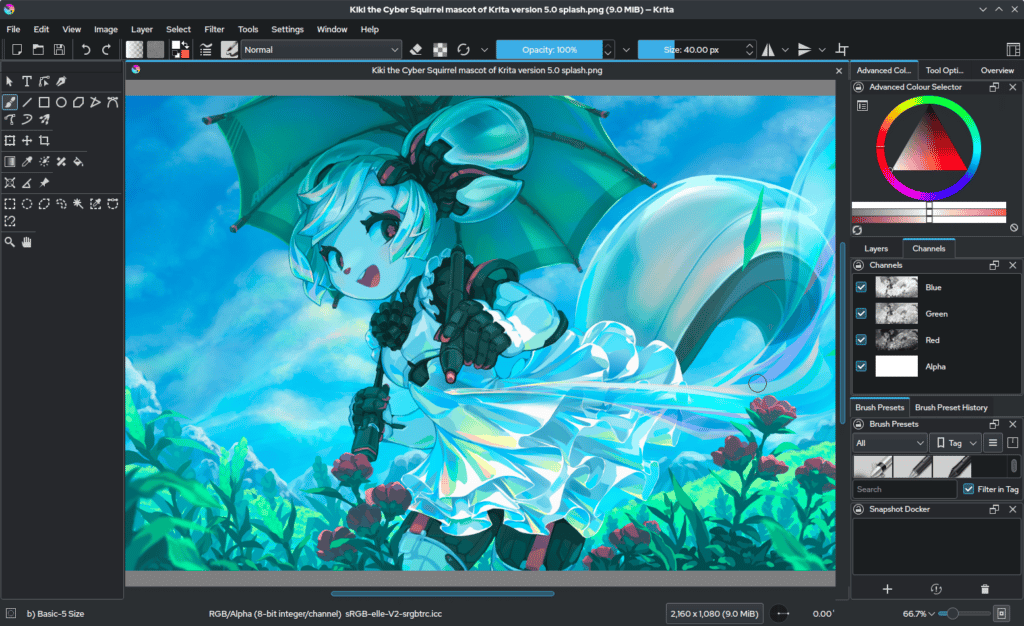
\includegraphics[height=4cm]{img/traditionaldigitalart}
	\caption{Example of a traditional digital drawing}
	\label{fig:traditionalart}
	\end{figure}	
	
	\item{3D Artwork} (\autoref{fig:3dart})
	
For a 3 dimension artwork we can take realistic video-games as an example . After a modeler makes shapes and creates a living world inside the computer, it's the artists job to give it life, paint it, change the textures, the sky, water, switch the shapes, etc. 3D artwork, meaning it's a 3 dimensional matrix and has to be viewed using a projector with prespective or other eletronical visual displays.

	\begin{figure}[h]
	\center
	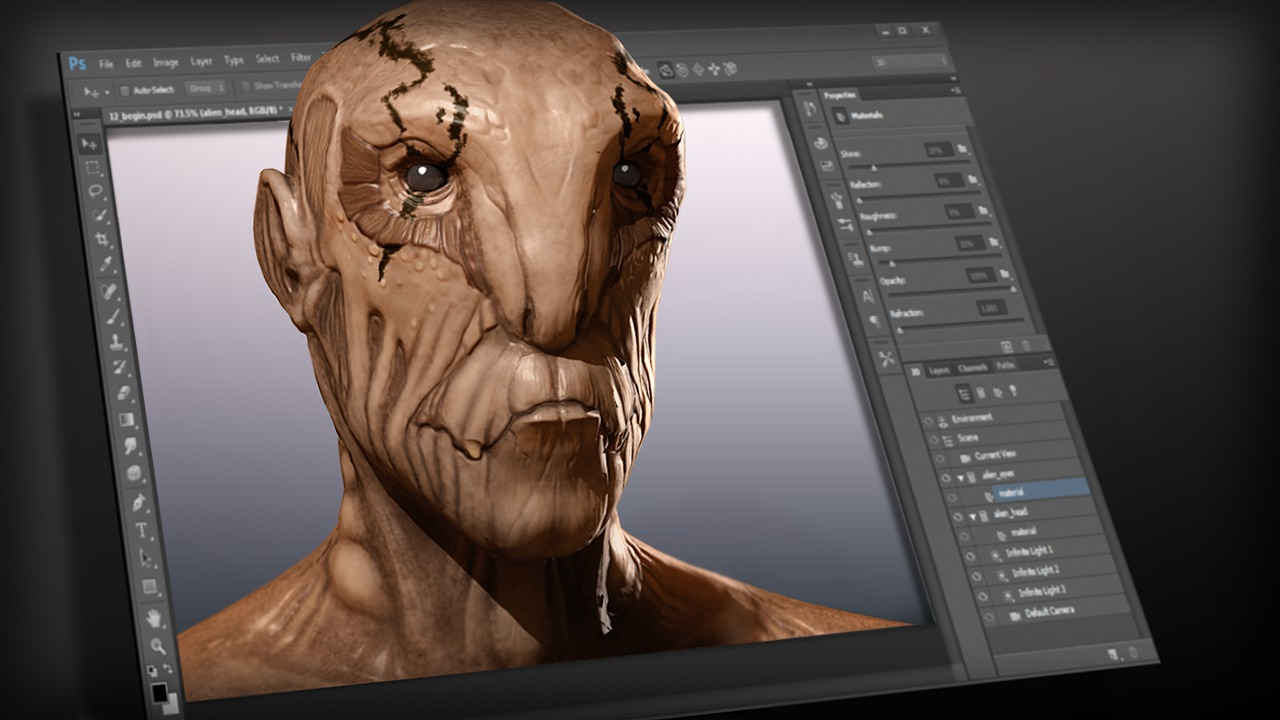
\includegraphics[height=5cm]{img/3ddigitalart}
	\caption{Example of a 3D model}
	\label{fig:3dart}
	\end{figure}	
	
	\item{Computer-generated images} (\autoref{fig:aiart})
	
Computer-generated images are images created by the computer itself with the help of artificial intelligence. For this work to happen, it has to take references from other artists which casues a lot of controversy nowadays. Artists claim computer-generated images are illegaly stealing their art, which is true, because the references that it uses - which are done by other artists - are being manipulated without their consent. If used legally, it can create brand new art used references and get really interesting results .

	\begin{figure}[h]
	\center
	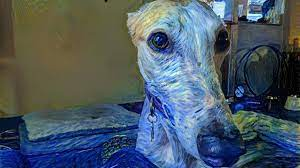
\includegraphics[height=4cm]{img/aiart}
	\caption{Example of a computed-generated artwork}
	\label{fig:aiart}
	\end{figure}	
	
	\item{Computer-generated animated imagery}
	
Computer-generated animated imagery is used extensively used nowadays in the entertainment field. Most, if not all series and movies we watch on a daily-basis use this kind of technique. The reason for this is because it provides the viewer with the best quality and experience while watching.
	
	\end{itemize}
 

\section{Pop art}

Pop art was an art movement born in England during the 50s. As capitalism was growing, artists wanted to make art more appealing to the masses, so they created and explored more ways to market their produts. During this era, all forms of art had just start becoming a part of our lives with the help of the media. The results of it's popularity, even if someone is not quite known about history, they can still identify works of art from this era since visuals became extravagant, dazzling and noticeable. It completely changed television, photography, comic books, cimena and advertising. 

Understanding Pop art is better with examples:
\begin{itemize}
	\item{Pop art in comic books} (\autoref{fig:comic})
	
We can conclude by observing \autoref{fig:comic} that comic books were heavily influenced by pop art. It was made to make a statement, exaggerate and it found it's true artistic expression for the first time during this era. It depicts a colorful fight between two jets in the sky.
	
	\begin{figure}[h]
	\center
	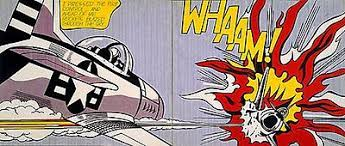
\includegraphics[height=4cm]{img/comic}
	\caption{Example of a comic book originated during this movement, "Whaam!", by Roy Lichtenstein}
	\label{fig:comic}
	\end{figure}	
	
	\item{Pop art influence over advertising} (\autoref{fig:advert})
	
It was during this movement that people combined commercialism and art, originating trends and the consumerism society.
	
	\begin{figure}[h]
	\center
	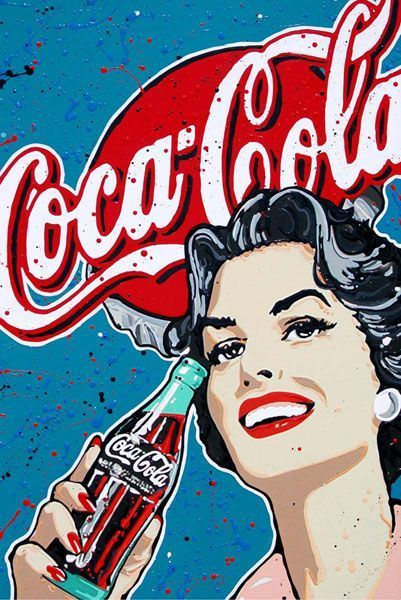
\includegraphics[height=4cm]{img/ad}
	\caption{Example of an ad developed during this movement}
	\label{fig:advert}
	\end{figure}	
		
\end{itemize}

\section{Minimalistic Art}

Minimalistic art was born in the United States of America in the late 50s. It's a branch of abstract expressionism art, it evolves around the concept of removing everything that isn't essential. Usually perceived as a visual form of art, we can get a better understanding of this movement's impact on sculpures. As we can see in \autoref{fig:broken}, we conclude the form of this piece of art is minimalistic because of it's geometric form, an attempt of making a piece of art as objective as possible.

	\begin{figure}[h]
	\center
	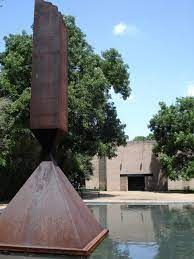
\includegraphics[height=6cm]{img/broken1}
	\caption{"Broken Obelisk" by Barnett Newman}
	\label{fig:broken}
	\end{figure}	
		
Minimalistic pieces can be characterized as pure and because it's the simplest form of beauty and it doesn't try to pretend to be anything it isn't. It's a radical way of expressing something objectively in the artistic world, the art you see in front of you is nothing more than the first perception you have from it.
This movement also had it's influence on paintings, which also resemble objective and geometric figures. 
The \autoref{fig:tmrs2} is a painting made by Frank Stella, a well known artists for being minimalistic. The painting is all black, leaving straight white lines untouched. Her famous quote “My painting is based on the fact that only what can be seen there is there… What you see is what you see” describes incredibly well every minimalistic piece of art. 
	
	\begin{figure}[h]
	\center
	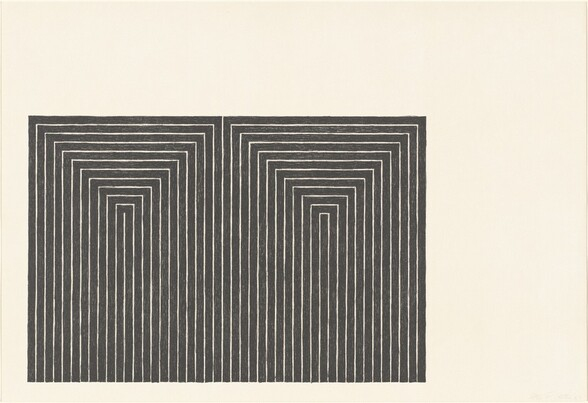
\includegraphics[height=6cm]{img/trms2}
	\caption{"The Marriage of Reason and Squalor, II" Frank Stella}
	\label{fig:tmrs2}
	\end{figure}	
		
Some of the most important painters during this era are:
\begin{itemize}
	\item{Ellsworth Kelly}
	\item{Agnes Martin}
	\item{Robert Ryman}
\end{itemize}
		
\section{Social Realism Art}

Social Realism Art was a movement created during the 20th century, marked by the social differences and the hard life of the working class. It's goal was to draw attention and bring change to the power structures by picturing the harsh truth of poverty after the Great Depression, caused by the excessive materilist trends, political corruption, labour-management conflicts, etc.	It origined between the two world wars and the artists did their best to make it more accessible by using mostly anonymous portraits of workers as the heroes of nations and hold the government and social systems accountable for the deteriorating conditions of the poor. During this movement, many projects were born in response for the depression lived during times of war, including:
\begin{itemize}

	\item{The Ashcan School}

The Ashcan School was a grouping of artists, not necessarily politically involved, who wanted to paint exactly the colors the daily life of the workforce. The group although popular, was not organized or unified. Even though the artists were interested and dedicated their work for this movement, they generaly did not share carear goals or political ideologies. The group included Robert Henri, John Sloan, George Bellows, William Glackens, Everett Shinn and many others. Some of their best work is in \autoref{fig:ashcan}


\begin{figure}[h]
\center
a) 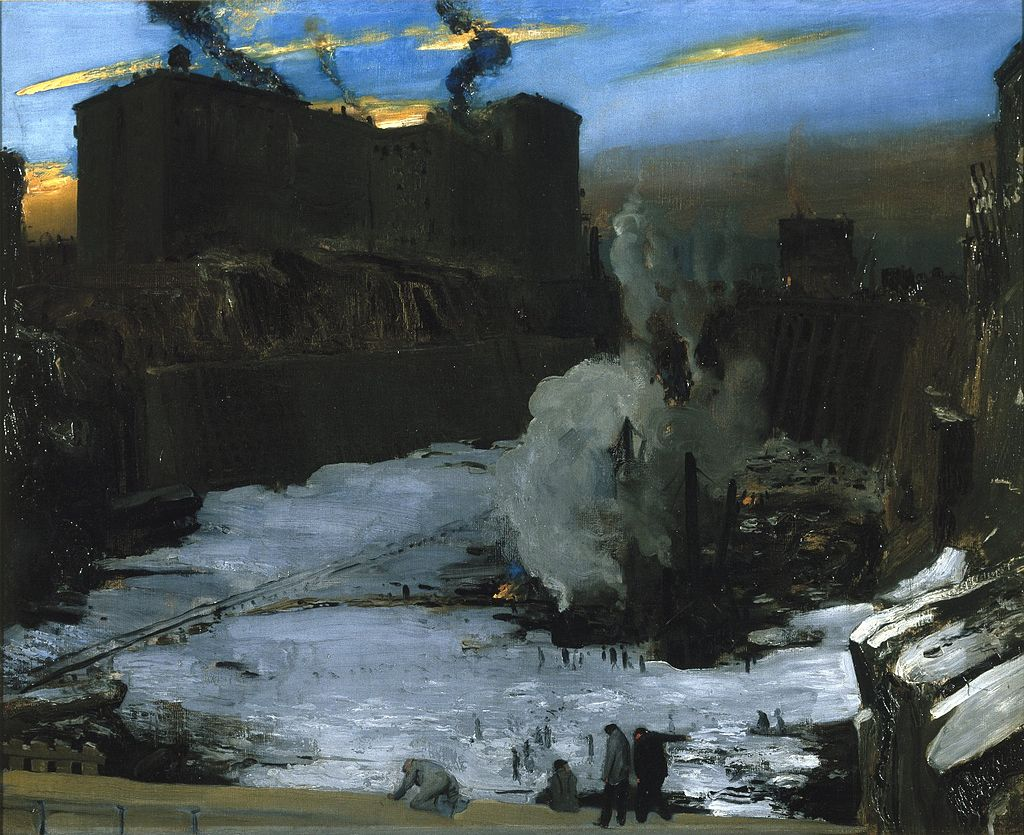
\includegraphics[height=3cm]{img/exca}
b) 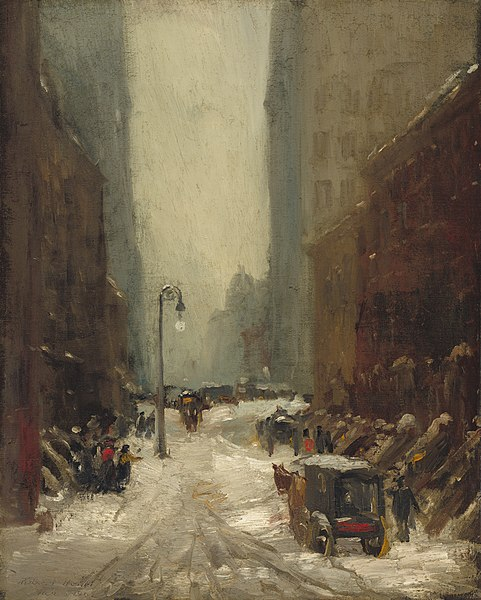
\includegraphics[height=3cm]{img/snow}
c) 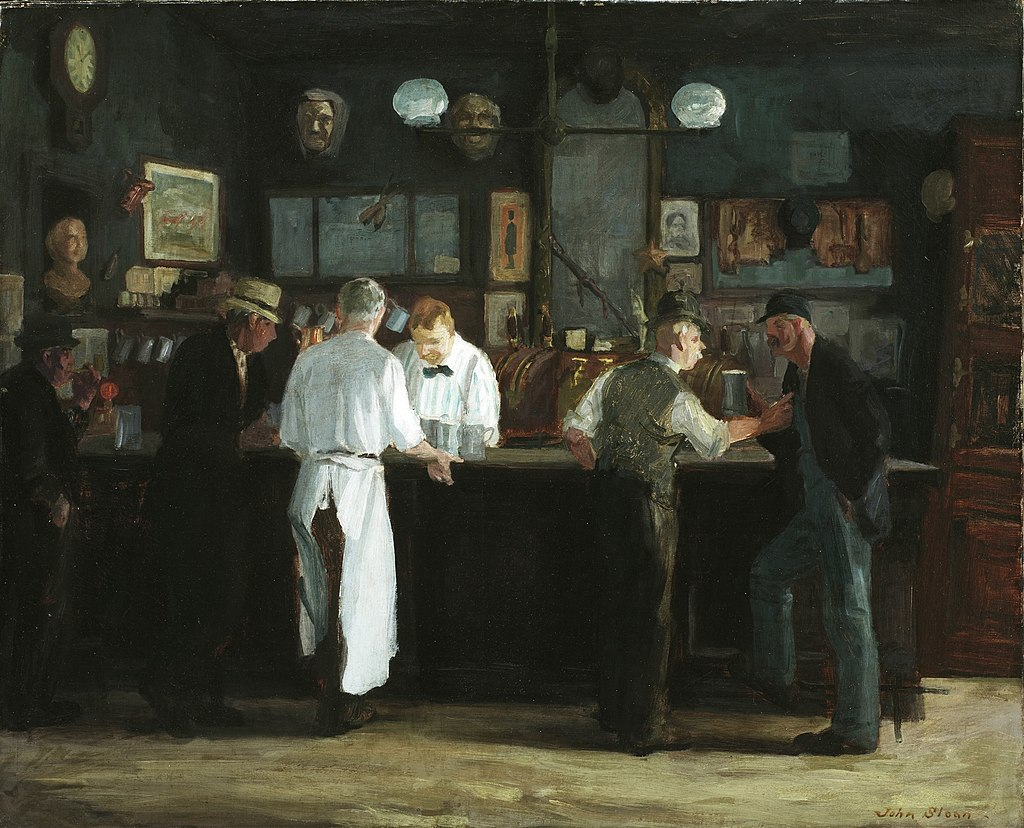
\includegraphics[height=3cm]{img/bar}
\caption{Examples of work from Ashcan members: a) "Pennsylvania Station Excavation" by George Bellows,
b) "Snow in New York" by Robert Henri, c) "McSorley's Bar" by John Sloan}
\label{fig:ashcan}
\end{figure}

	\item{Farm Security Administration Project}
	
The great Depression was marked with overproduction, mechanization and failing prices, triggering a lot of farm labourers into unemployment and businesses into bankrupcy.
After Franklin Roosevelt took power in the USA after 1933, he created a series of programs as a solution to bring the country out of Depression - \textbf{the New Deal} - and it included Civilian Conservation Corps, the Works Progress Administration, the Civil Works Administration, \textbf{the Farm Security Administration}, the National Industrial Recovery Act of 1933 and the Social Security Administration.
Farm Security Administration project commissioned photographers to take proof of the living conditions of farmers. It resulted on a huge 80000 picture document (\cite{WEBSITE:2}). Some of the most popular photos taken for this project are in \autoref{fig:fsaproject}.


\begin{figure}[h]
\center
a) 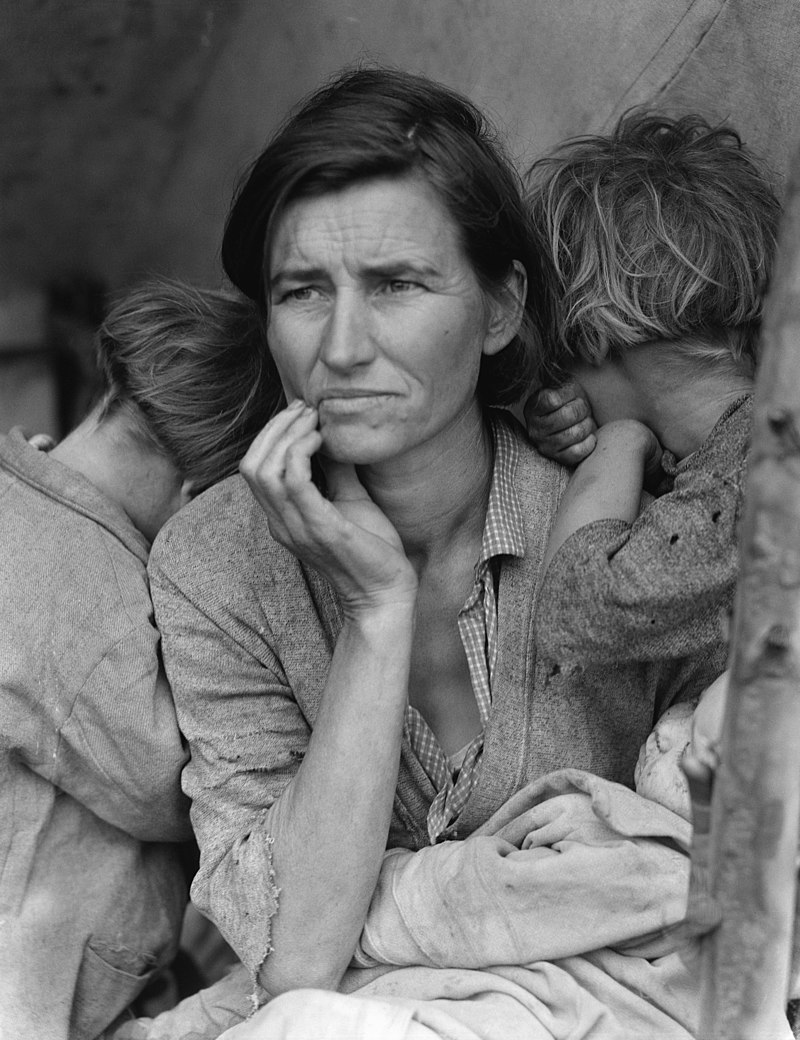
\includegraphics[height=3cm]{img/migrantmother}
b) 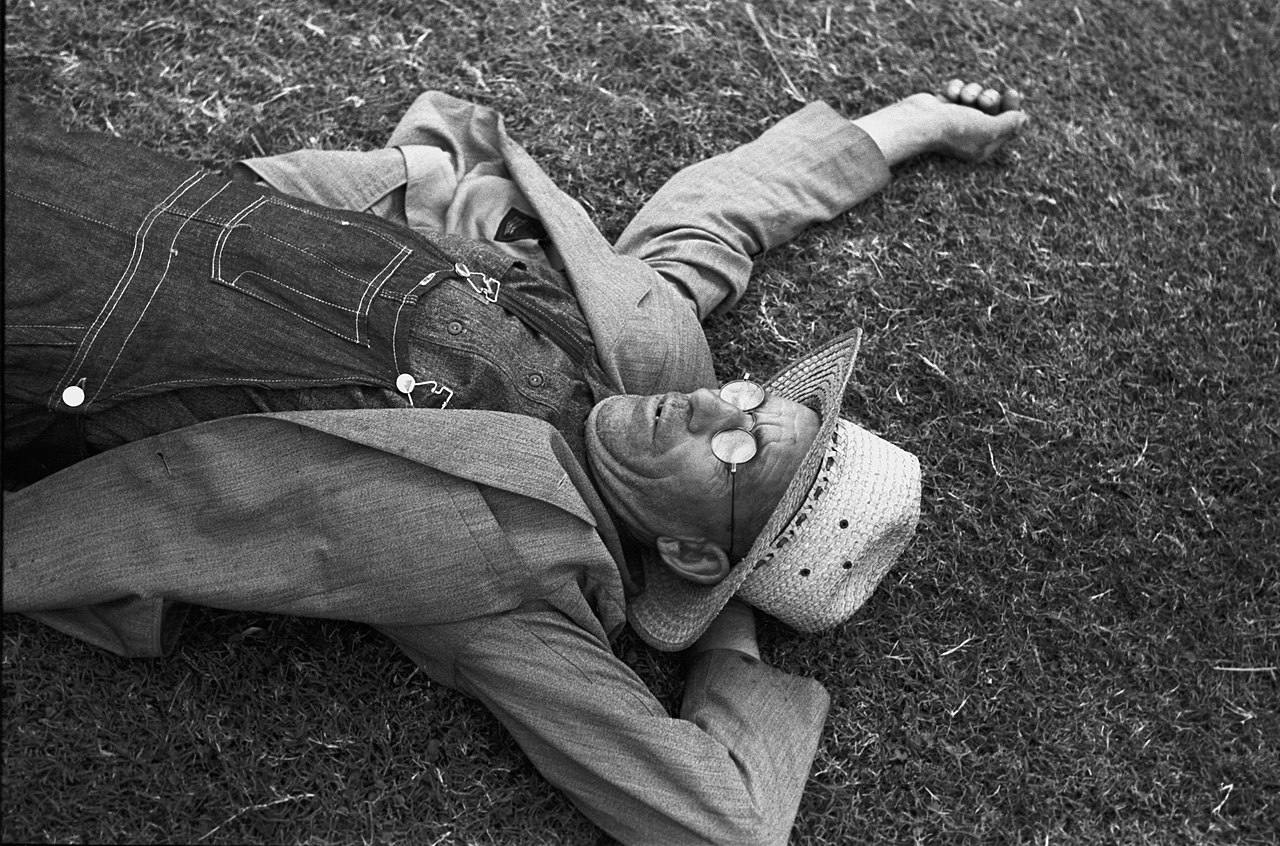
\includegraphics[height=3cm]{img/restingfarmer}
c) 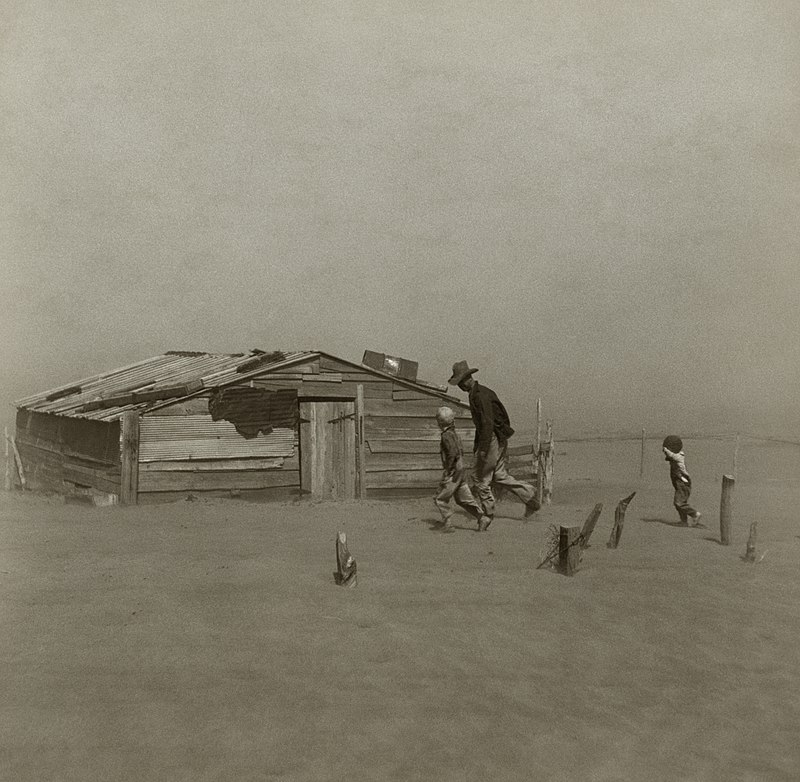
\includegraphics[height=3cm]{img/dust}
\caption{a) The iconic "Migrant Mother" photo, by Dorothea Lange, b) "Resting Farmer" by Russel Lee and c) "Dust Bowl Cimarron County, Oklahoma" by Arthur Rothstein}
\label{fig:fsaproject}
\end{figure}

\end{itemize}

\chapter{Conclusions}
\label{chap.conclusions}

After conducting this report, it can be concluded how important art is. We first explore what are some types of art, what it means to create paintings, how people show their emotions and values in three dimensions using different materials and creation techniques in sculptures, the cultural and heritage of humanity present in architecture, the progression and development of technology in photography and finally, the vocal and instrumental sounds which we categorize as music.

Picasso and other cubists rocked the world changing the established rules of using perspective and spacial concepts, The works of Leonardo da Vinci's and it's influence over the world until today during the Renaissance era, Surrealists put dreams on canvas forming abstract and unreal compositions, which had an element of absurdity, Impressionists such as Renoir, Degas and Monet blurred the line between fiction and reality using the shadow and light. Expressionism concentrated on showing the true nature of man and its strong feelings like anxiety or tension. 

Then focus was on exploration of street artists, who create murals, graffiti, tags or stickers group in public spaces ignoring rules and constraints, the digital art era, which was provided by new technology and gave artists hundreds of new possibilities and accessibility, the influence of Pop art on a materialistic society and the creation of trends to make art more appealing to the masses, the raw, true and pure aspect of Minimalistic art, based on appreciating art qualified as basic and in last, Social Realism which brought attention to the heroic working class, their poverty and hard working life during poverty, war and corruption.


\chapter*{Authors contributions}
Choosing the topic, creation of chapters, filling section Authors contributions, conclusions. \ac{rr}, \ac{zs}

Introduction chapter and sections: Sculpture, Architecture, Impressionism, Expressionism, Surrealism, Cubism, Street Art. \ac{zs}

Abstract, sections: Painting, Photography, Music, Renaissance, Digital Art, Pop Art, Minimalistic Art, Social Realism Art. \ac{rr}

\vspace{10pt}

\authors : 50\%, 50\%.\\

%%%%%%%%%%%%%%%%%%%%%%%%%%%%%%%%%
\chapter*{Acronyms}
\begin{acronym}
\acro{rr}[RR]{Rodrigo Ribeiro}
\acro{zs}[ZS]{Zuzanna Sikorska}
\end{acronym}


%%%%%%%%%%%%%%%%%%%%%%%%%%%%%%%%%
\printbibliography

\end{document}
